\section*{Step 3}

\begin{custombox}[label={box:Q3}]{Step 3}
	Use the following algorithms to cluster the observations is each of the dataset. Plot the outcomes.
	\begin{enumerate}[label=\alph*.]
		\item K-Means Clustering
		\item Agglomerative Clustering
		\item DBSCAN
	\end{enumerate}
\end{custombox}

Here, we will use three clustering algorithms to cluster the observations in each dataset. We will plot the outcomes to visualize the clustering results.

\begin{lstlisting}[language=Python, caption=Code to Cluster Datasets and generate Metrics]
def plot_clusters(data, labels, title, name):
    plt.figure(figsize=(16, 10))
    plt.scatter(data[:, 0], data[:, 1], c=labels, cmap='viridis', s=40, edgecolors='black')
    plt.title(title)
    plt.xlabel('x1')
    plt.ylabel('x2')
    plt.savefig(f'Images/{name}-{title}.png', dpi=400)
    plt.show()

def run_clustering(data, name):
    results = []
    
    kmeans = KMeans(n_clusters=4, random_state=42)
    kmeans_labels = kmeans.fit_predict(data)
    plot_clusters(data, kmeans_labels, 'K-Means Clustering', name)
    kmeans_metrics = [
        'KMeans',
        silhouette_score(data, kmeans_labels),
        calinski_harabasz_score(data, kmeans_labels),
        davies_bouldin_score(data, kmeans_labels)
    ]
    results.append(kmeans_metrics)

    agglomerative = AgglomerativeClustering(n_clusters=4)
    agglomerative_labels = agglomerative.fit_predict(data)
    plot_clusters(data, agglomerative_labels, 'Agglomerative Clustering', name)
    agglomerative_metrics = [
        'AgglomerativeClustering',
        silhouette_score(data, agglomerative_labels),
        calinski_harabasz_score(data, agglomerative_labels),
        davies_bouldin_score(data, agglomerative_labels)
    ]
    results.append(agglomerative_metrics)

    linkage_matrix = linkage(data, method='ward')

    plt.figure(figsize=(16, 10))
    plt.title('Dendrogram for Agglomerative Clustering')
    plt.xlabel('Sample Index')
    plt.ylabel('Distance')
    plot_dendrogram(linkage_matrix, truncate_mode='level', p=4)
    plt.savefig(f'Images/{name}-Agglomerative-Dendrogram.png', dpi=400)
    plt.show()

    # eps_values = np.linspace(0.01, 4, 200)
    # min_samples_values = range(4, 21)

    best_dbscan_labels = None
    best_dbscan_score = -np.inf
    best_eps, best_min_samples = None, None

    if name == 'Clusters-5-v0':
        eps = 0.3107537688442211
        min_samples = 9
    elif name == 'Clusters-5-v1':
        eps = 0.23055276381909548
        min_samples = 20
    elif name == 'Clusters-5-v2':
        eps = 0.17040201005025127
        min_samples = 13

    # I found this 3 best_eps_values after running the dataset multiple times and checking the best silhouette score

    dbscan = DBSCAN(eps=eps, min_samples=min_samples)
    dbscan_labels = dbscan.fit_predict(data)
    best_dbscan_labels = dbscan_labels
    best_dbscan_score = silhouette_score(data, dbscan_labels)
    best_eps = eps
    best_min_samples = min_samples

    if best_dbscan_labels is not None:
        plot_clusters(data, best_dbscan_labels, 'DBSCAN Clustering', name)
        dbscan_metrics = [
            'DBSCAN',
            best_dbscan_score,
            calinski_harabasz_score(data, best_dbscan_labels),
            davies_bouldin_score(data, best_dbscan_labels)
        ]
        print(f"Best DBSCAN parameters: eps={best_eps}, min_samples={best_min_samples}")
    else:
        dbscan_metrics = ['DBSCAN', 'N/A', 'N/A', 'N/A']
        print("DBSCAN could not find exactly 4 clusters.")
    
    results.append(dbscan_metrics)

    result_df = pd.DataFrame(results, columns=['Algorithm', 'Silhouette Score', 'Calinski-Harabasz Score', 'Davies-Bouldin Score'])
    result_df.to_csv(f'Metrics/{name}-metrics.csv', index=False)

    plt.figure(figsize=(16, 10))
    plt.plot(result_df['Algorithm'], result_df['Silhouette Score'], marker='o', label='Silhouette Score')
    plt.plot(result_df['Algorithm'], result_df['Calinski-Harabasz Score'], marker='o', label='Calinski-Harabasz Score')
    plt.plot(result_df['Algorithm'], result_df['Davies-Bouldin Score'], marker='o', label='Davies-Bouldin Score')
    plt.title(f'Metrics for {name}')
    plt.yscale('log')
    plt.ylabel('Score (Log Scale)')
    plt.xlabel('Algorithm')
    plt.legend()
    plt.savefig(f'Metrics/{name}-metrics.png', dpi=400)
    plt.show()

    return results

for name, data in dataset.items():
    scaled_data = scalers[name]
    clustering_results = run_clustering(scaled_data, name)

\end{lstlisting}

\begin{figure}[H]
	\centering
	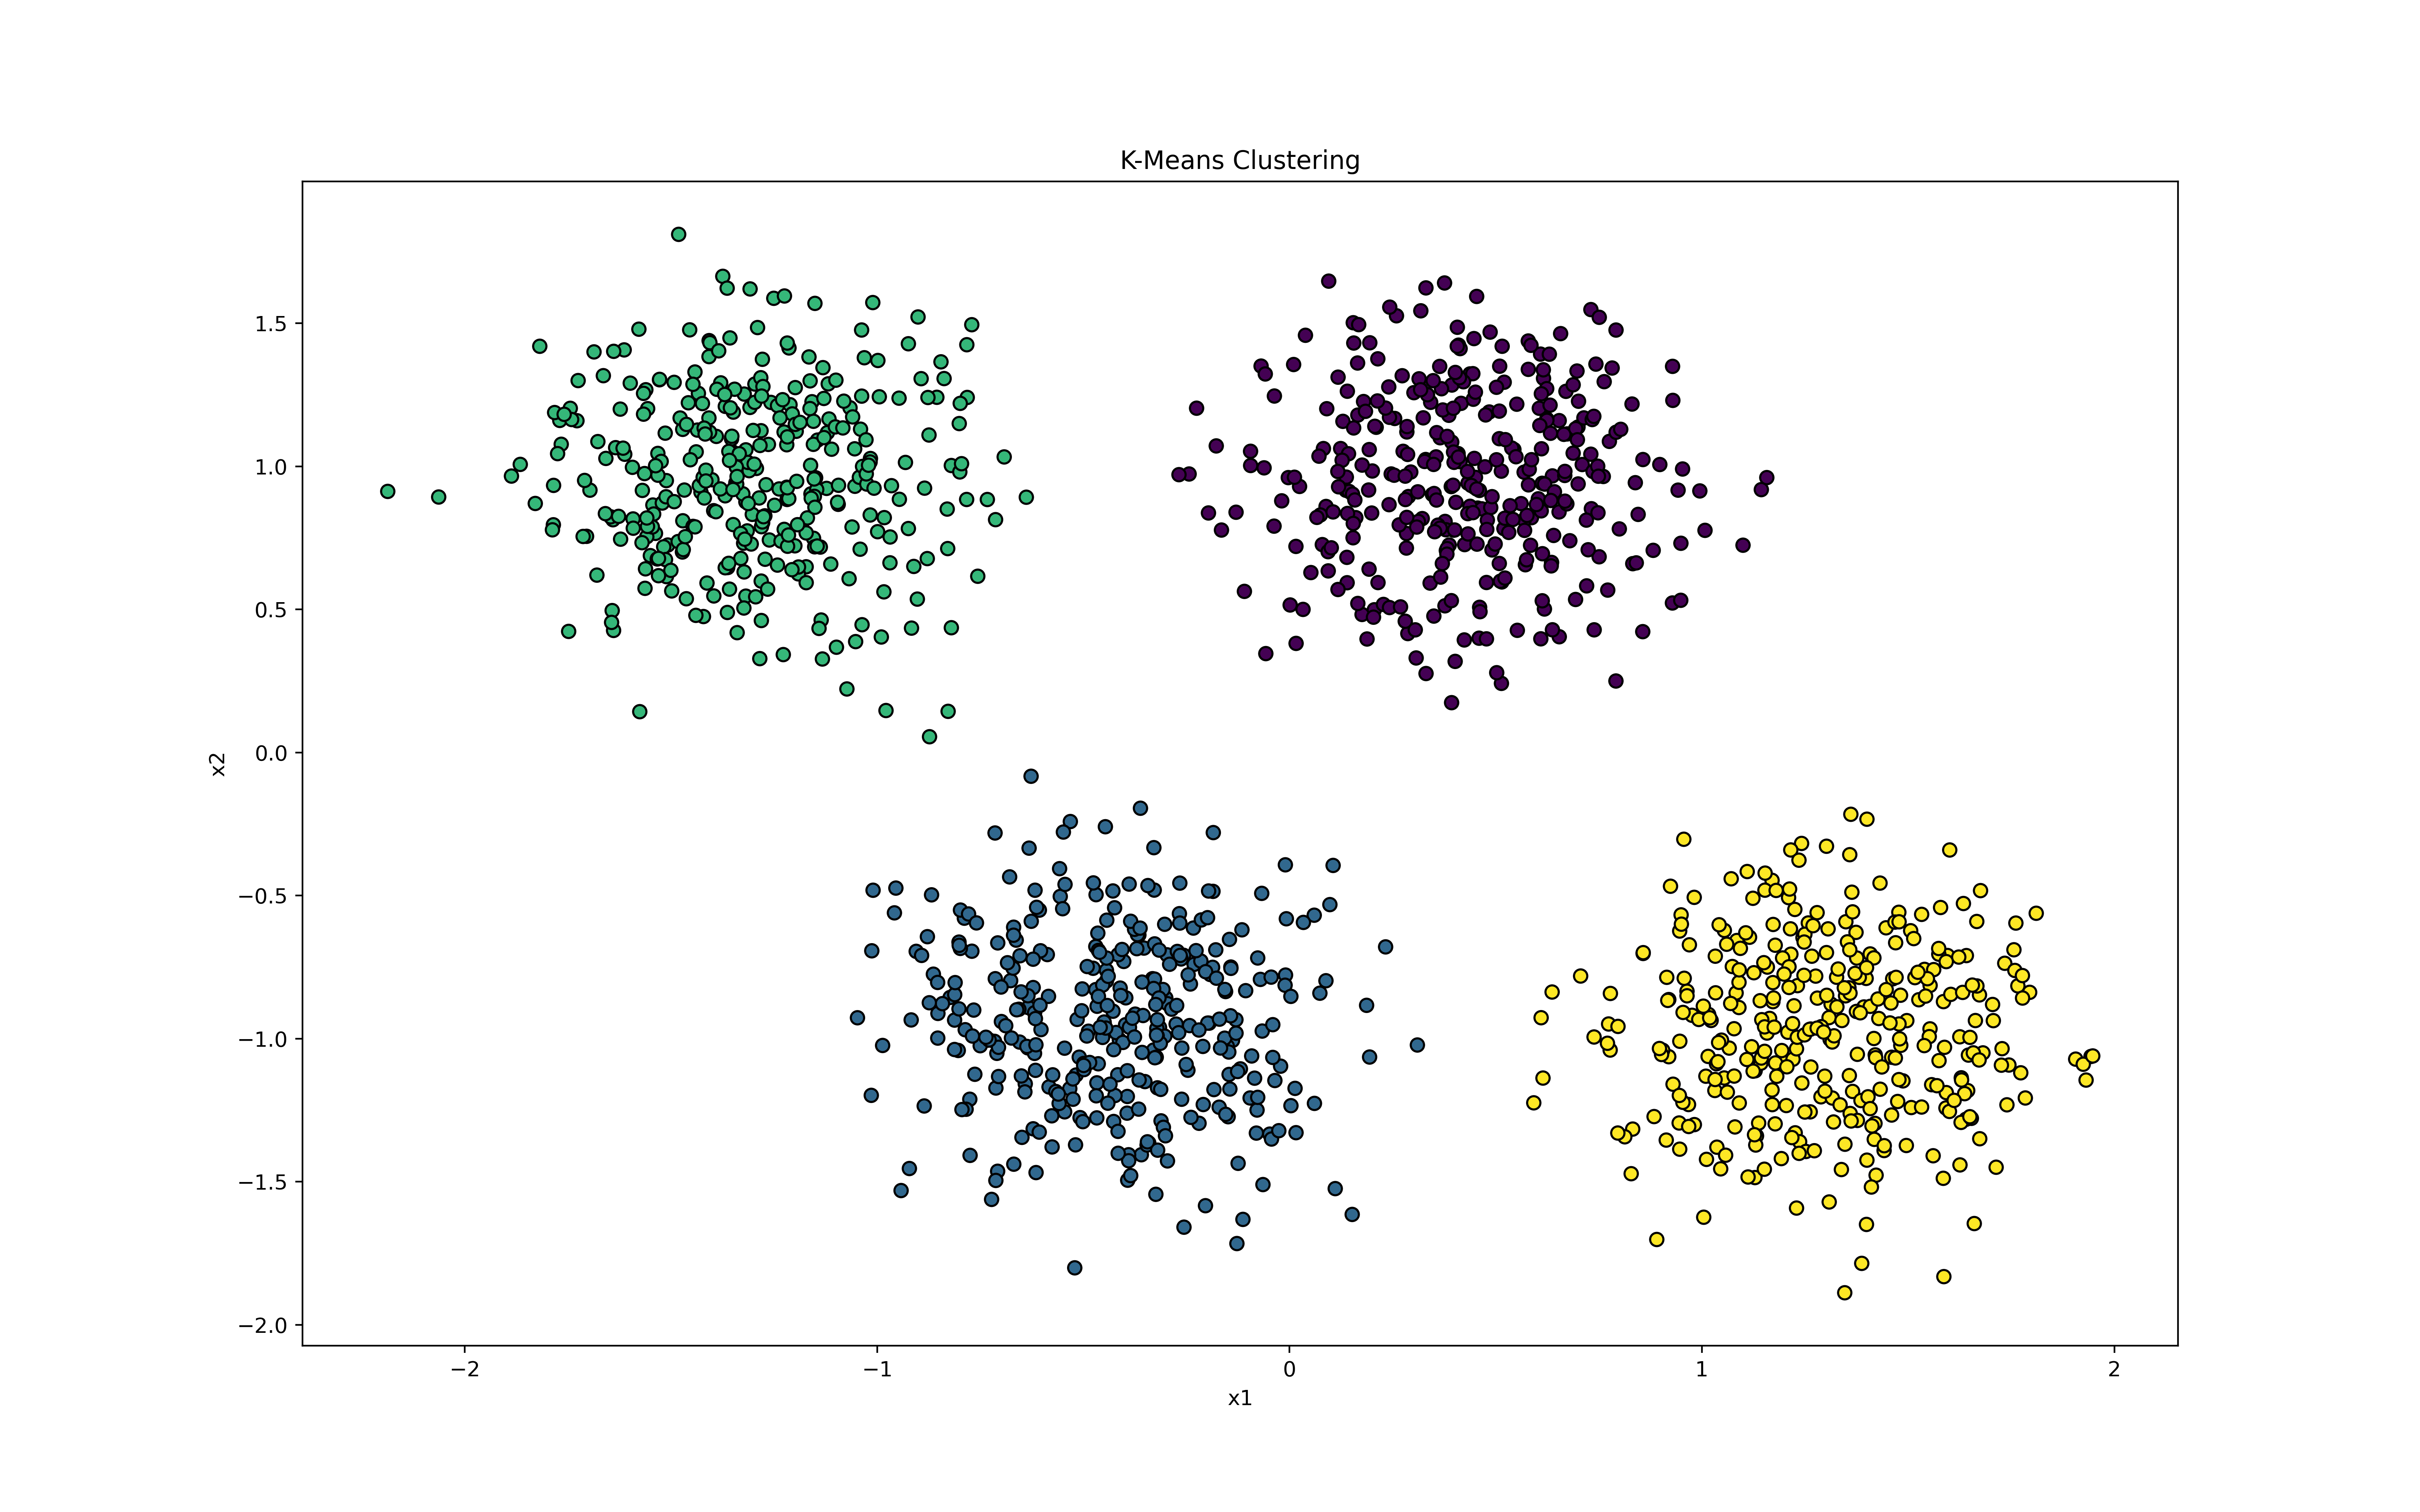
\includegraphics[width=0.9\linewidth]{Images/Clusters-5-v0-K-Means Clustering.png}
	\caption{Dataset 1: K-Means Clustering}
	\label{fig:clusters-5-v0-k-means-clustering}
\end{figure}

\begin{figure}[H]
	\centering
	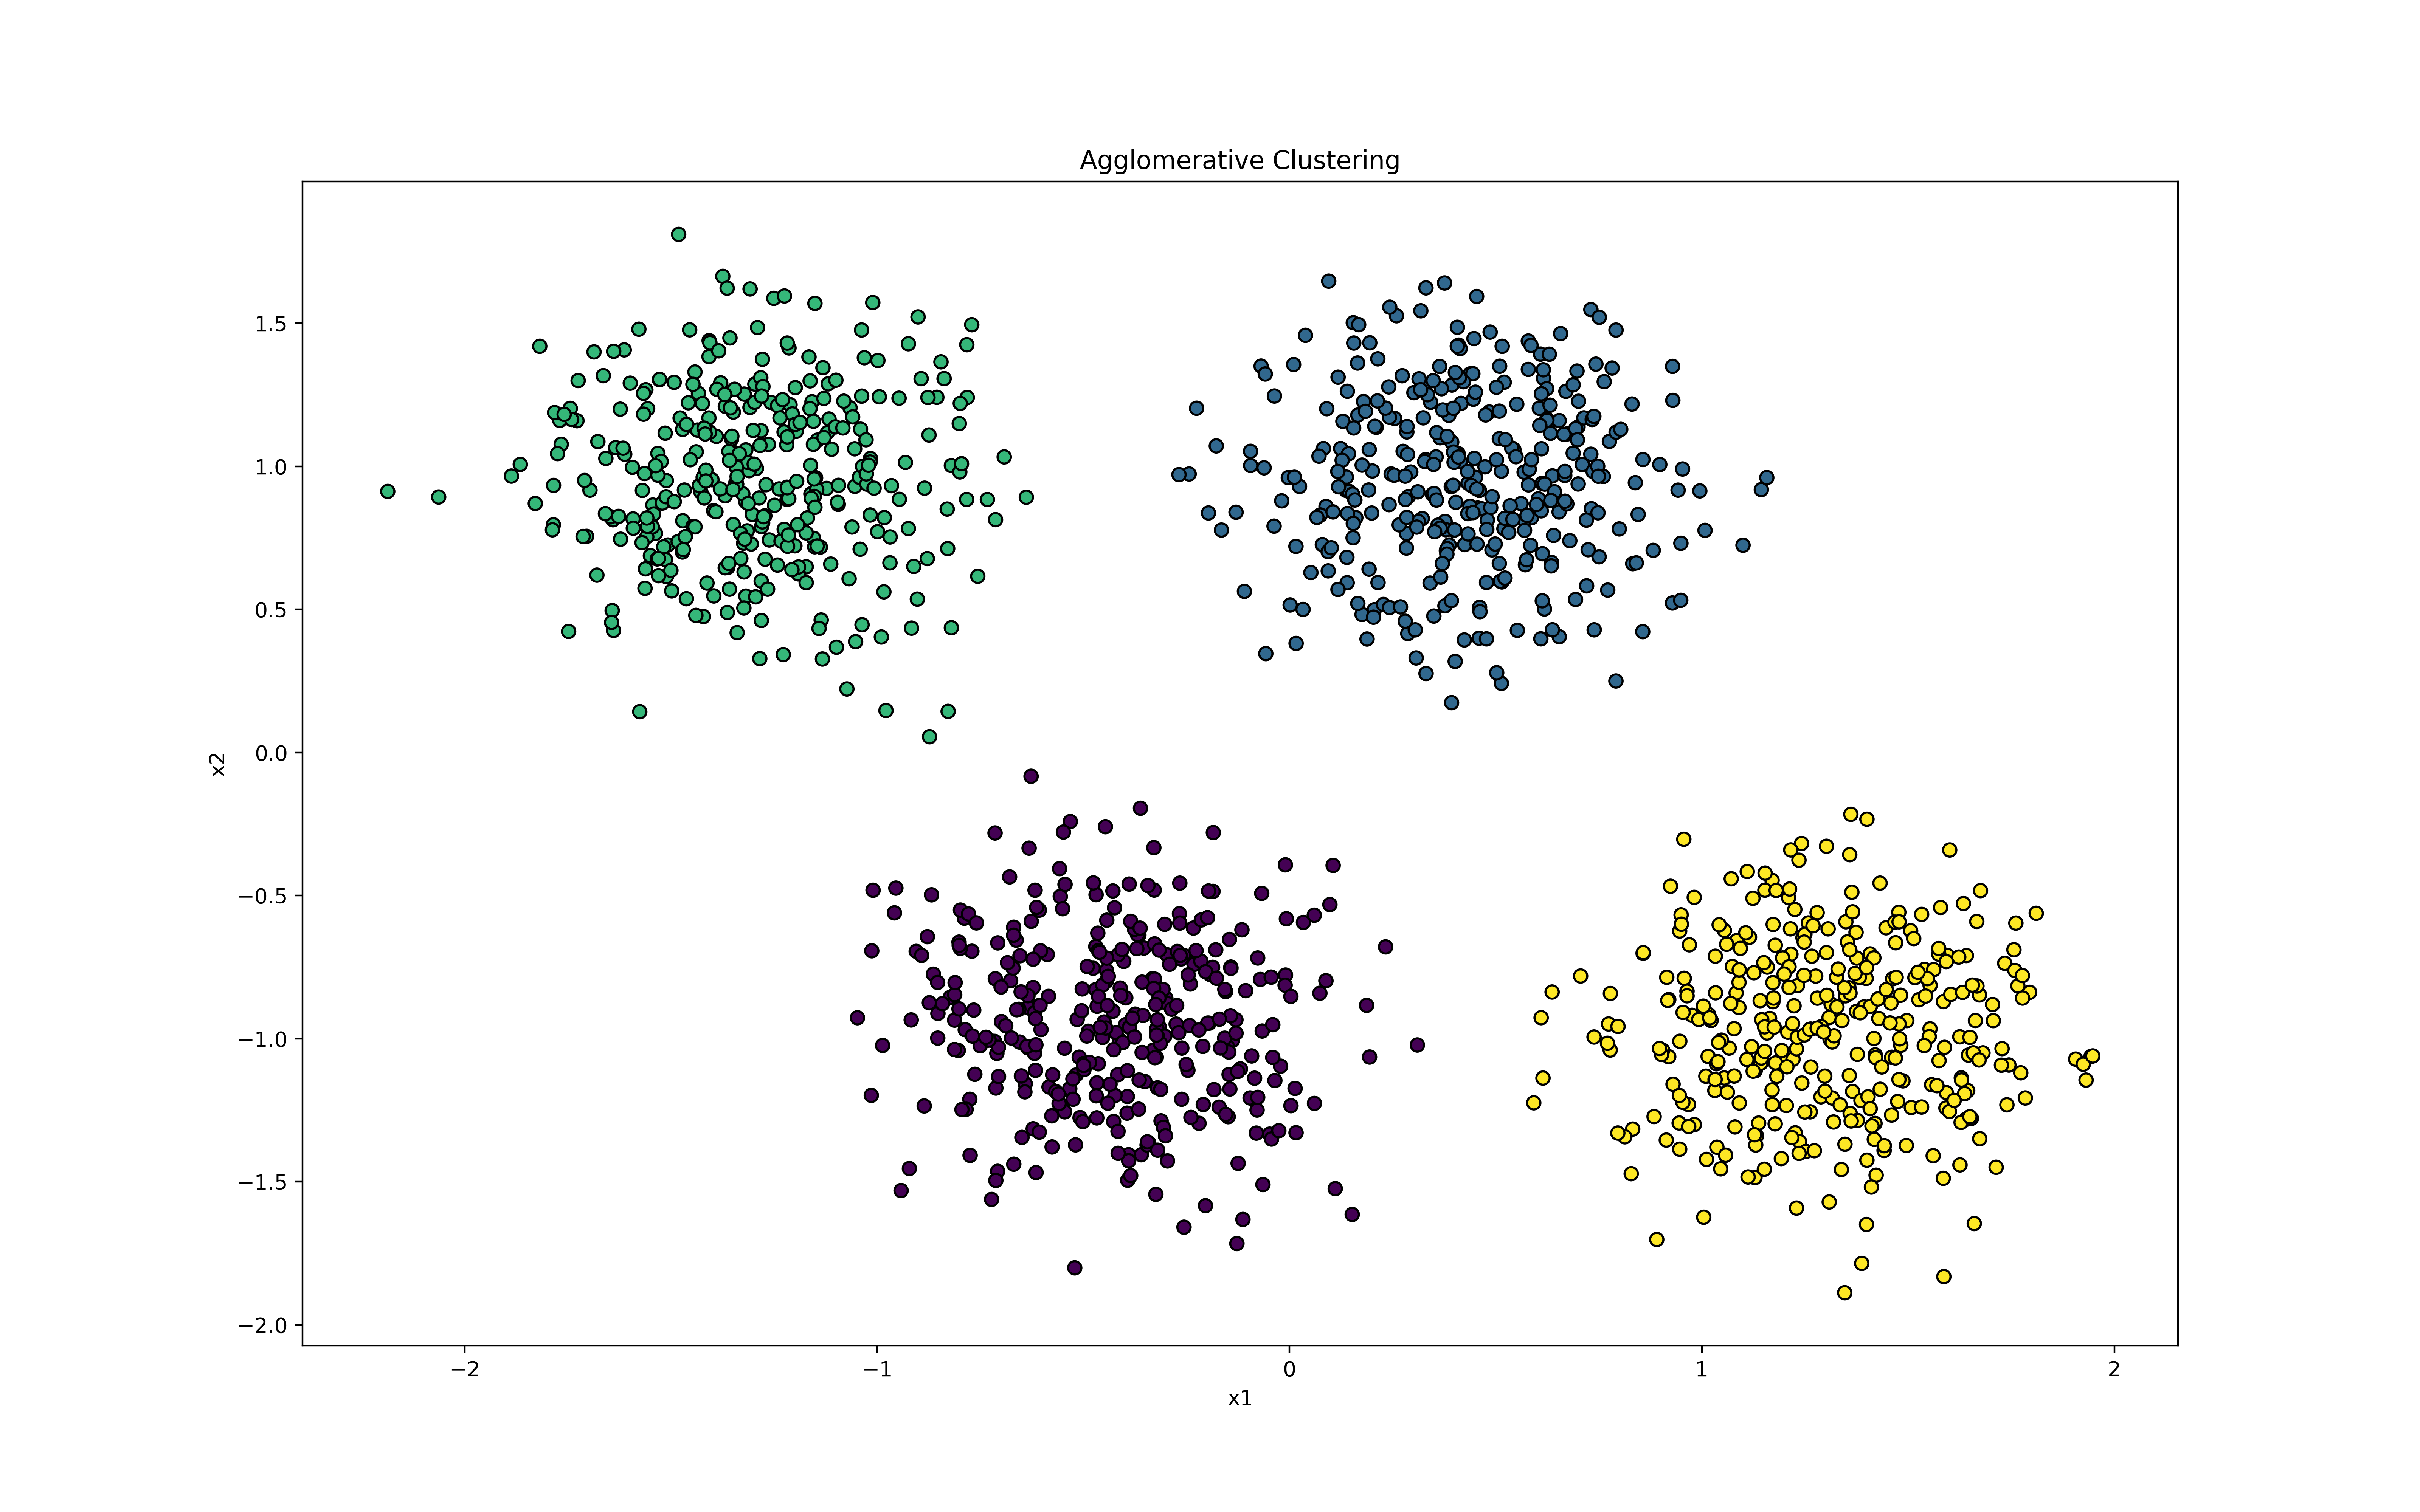
\includegraphics[width=0.9\linewidth]{Images/Clusters-5-v0-Agglomerative Clustering.png}
	\caption{Dataset 1: Agglomerative Clustering}
	\label{fig:clusters-5-v0-agglomerative-clustering}
\end{figure}

\begin{figure}[H]
    \centering
    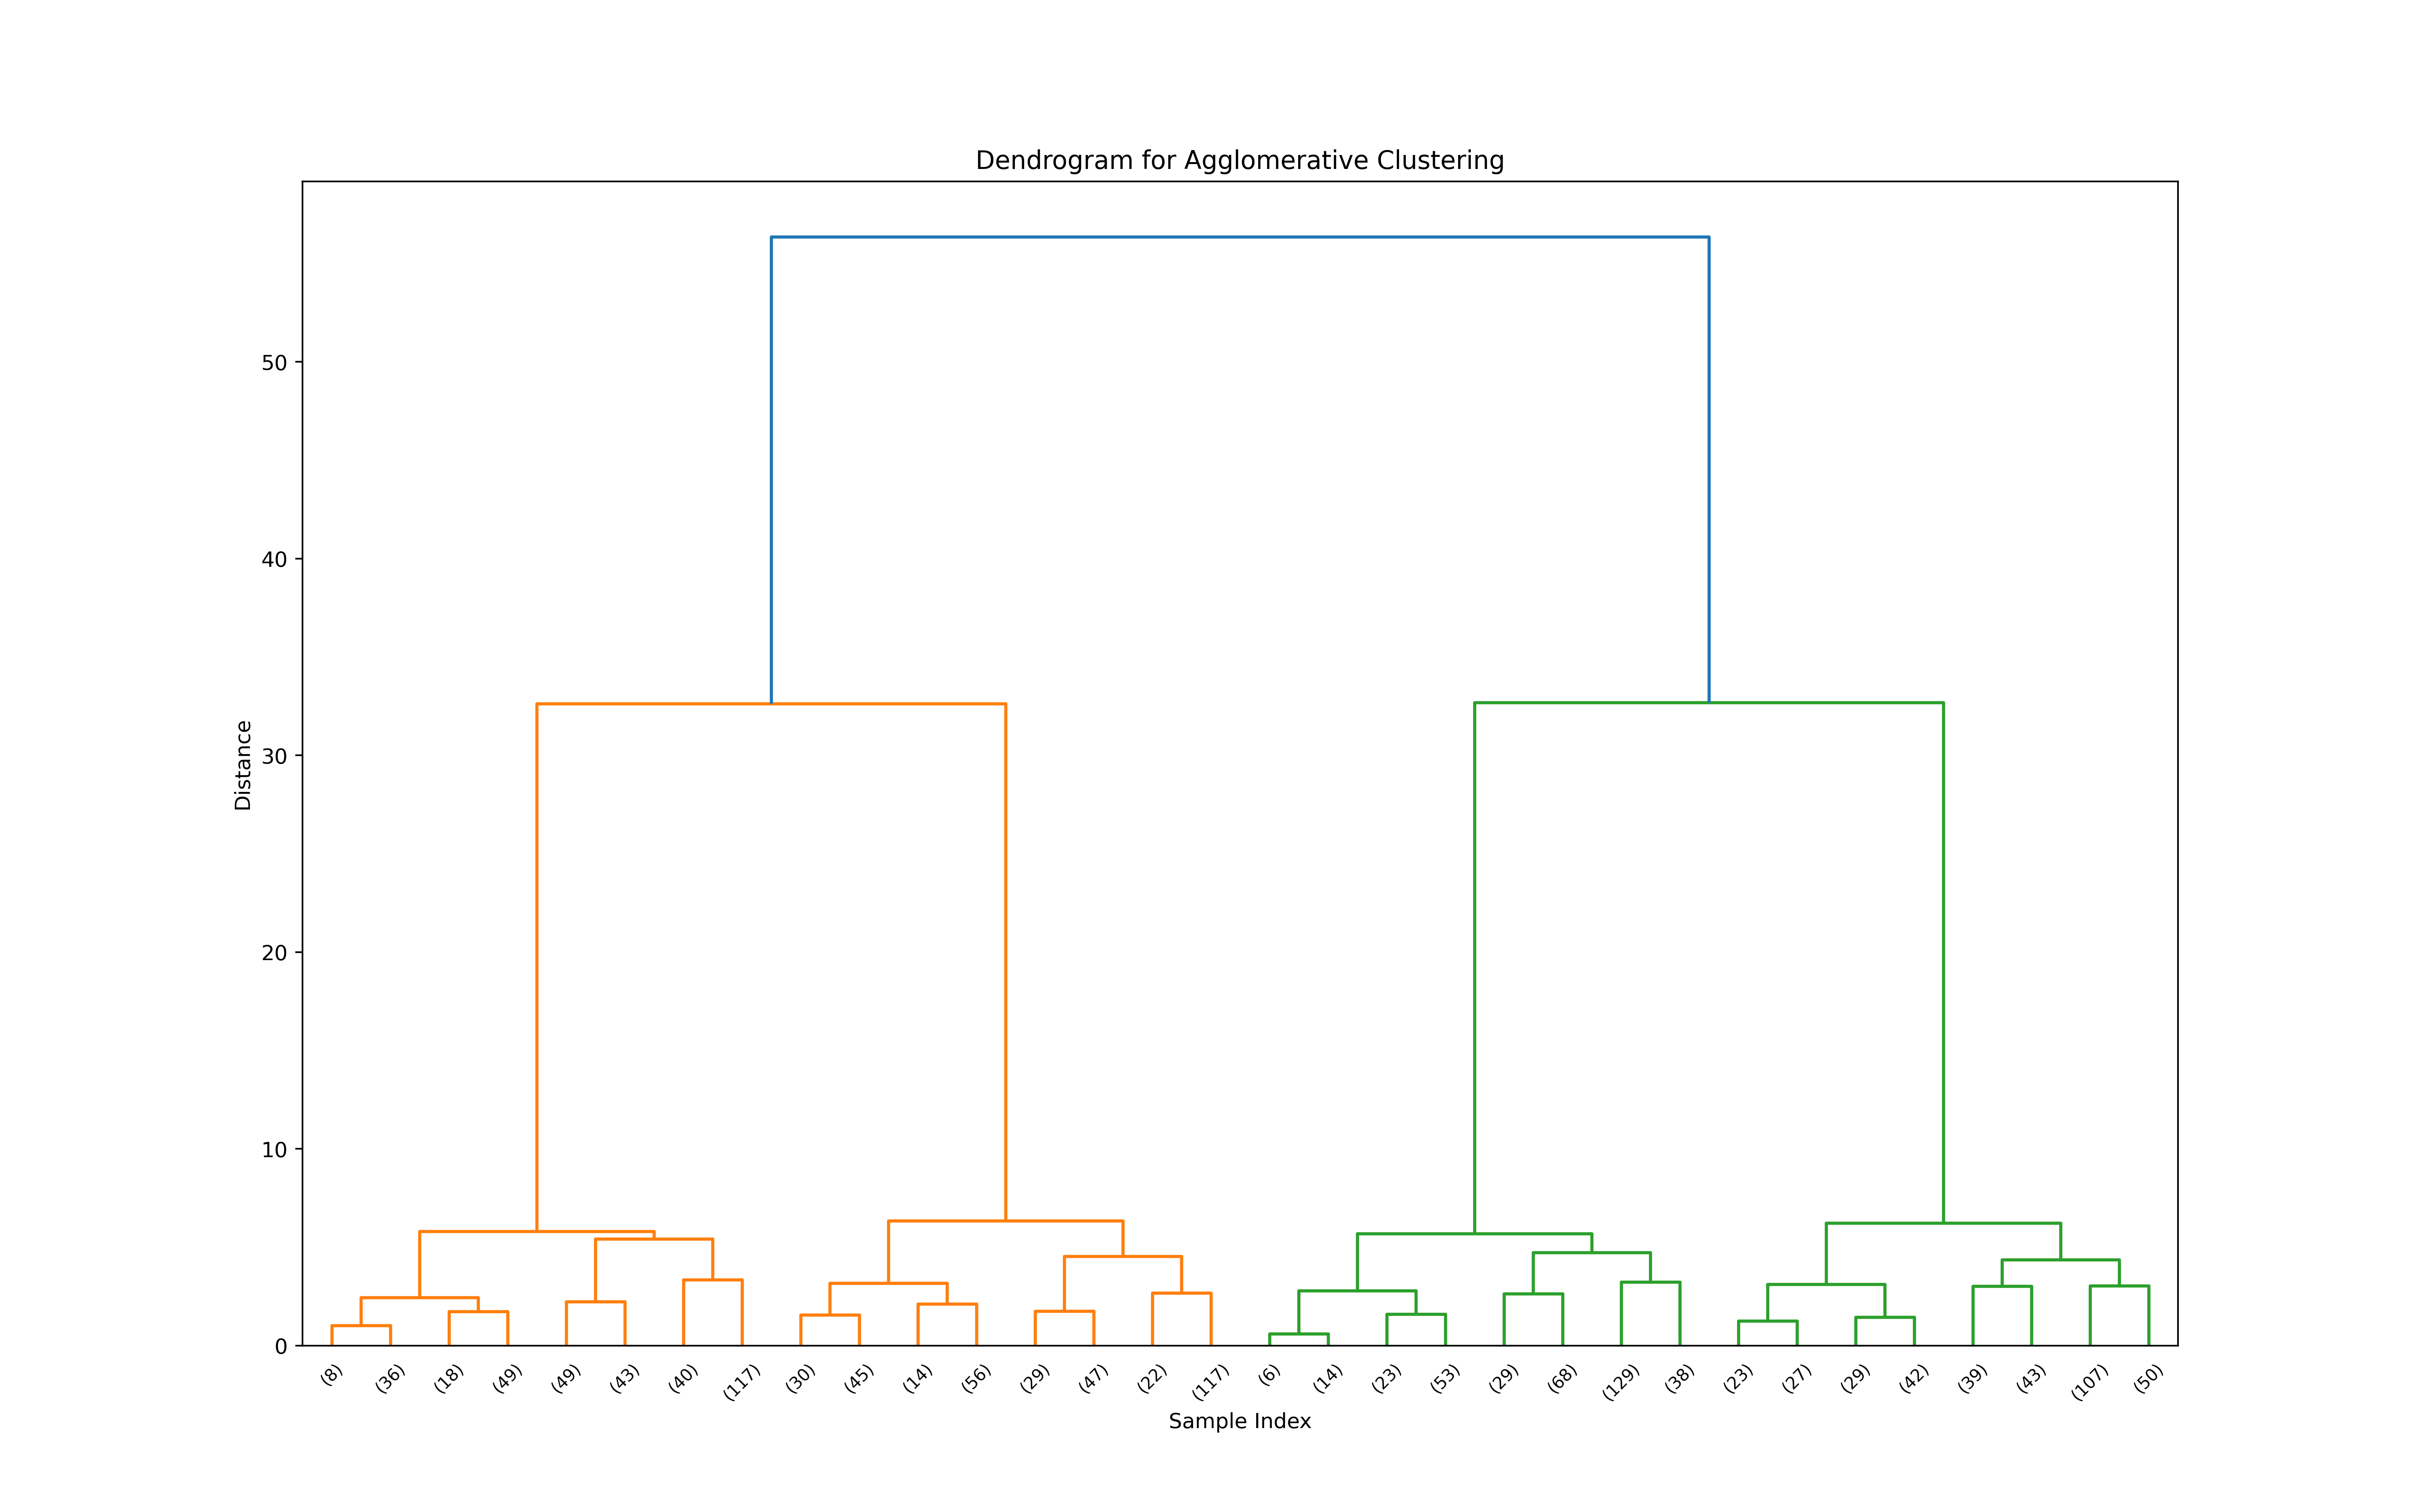
\includegraphics[width=0.75\linewidth]{Images/Clusters-5-v0-Agglomerative-Dendrogram.png}
    \caption{Dataset 1: Agglomerative Clustering Dendrogram}
    \label{fig:clusters-5-v0-agglomerative-dendrogram}
\end{figure}

\begin{figure}[H]
	\centering
	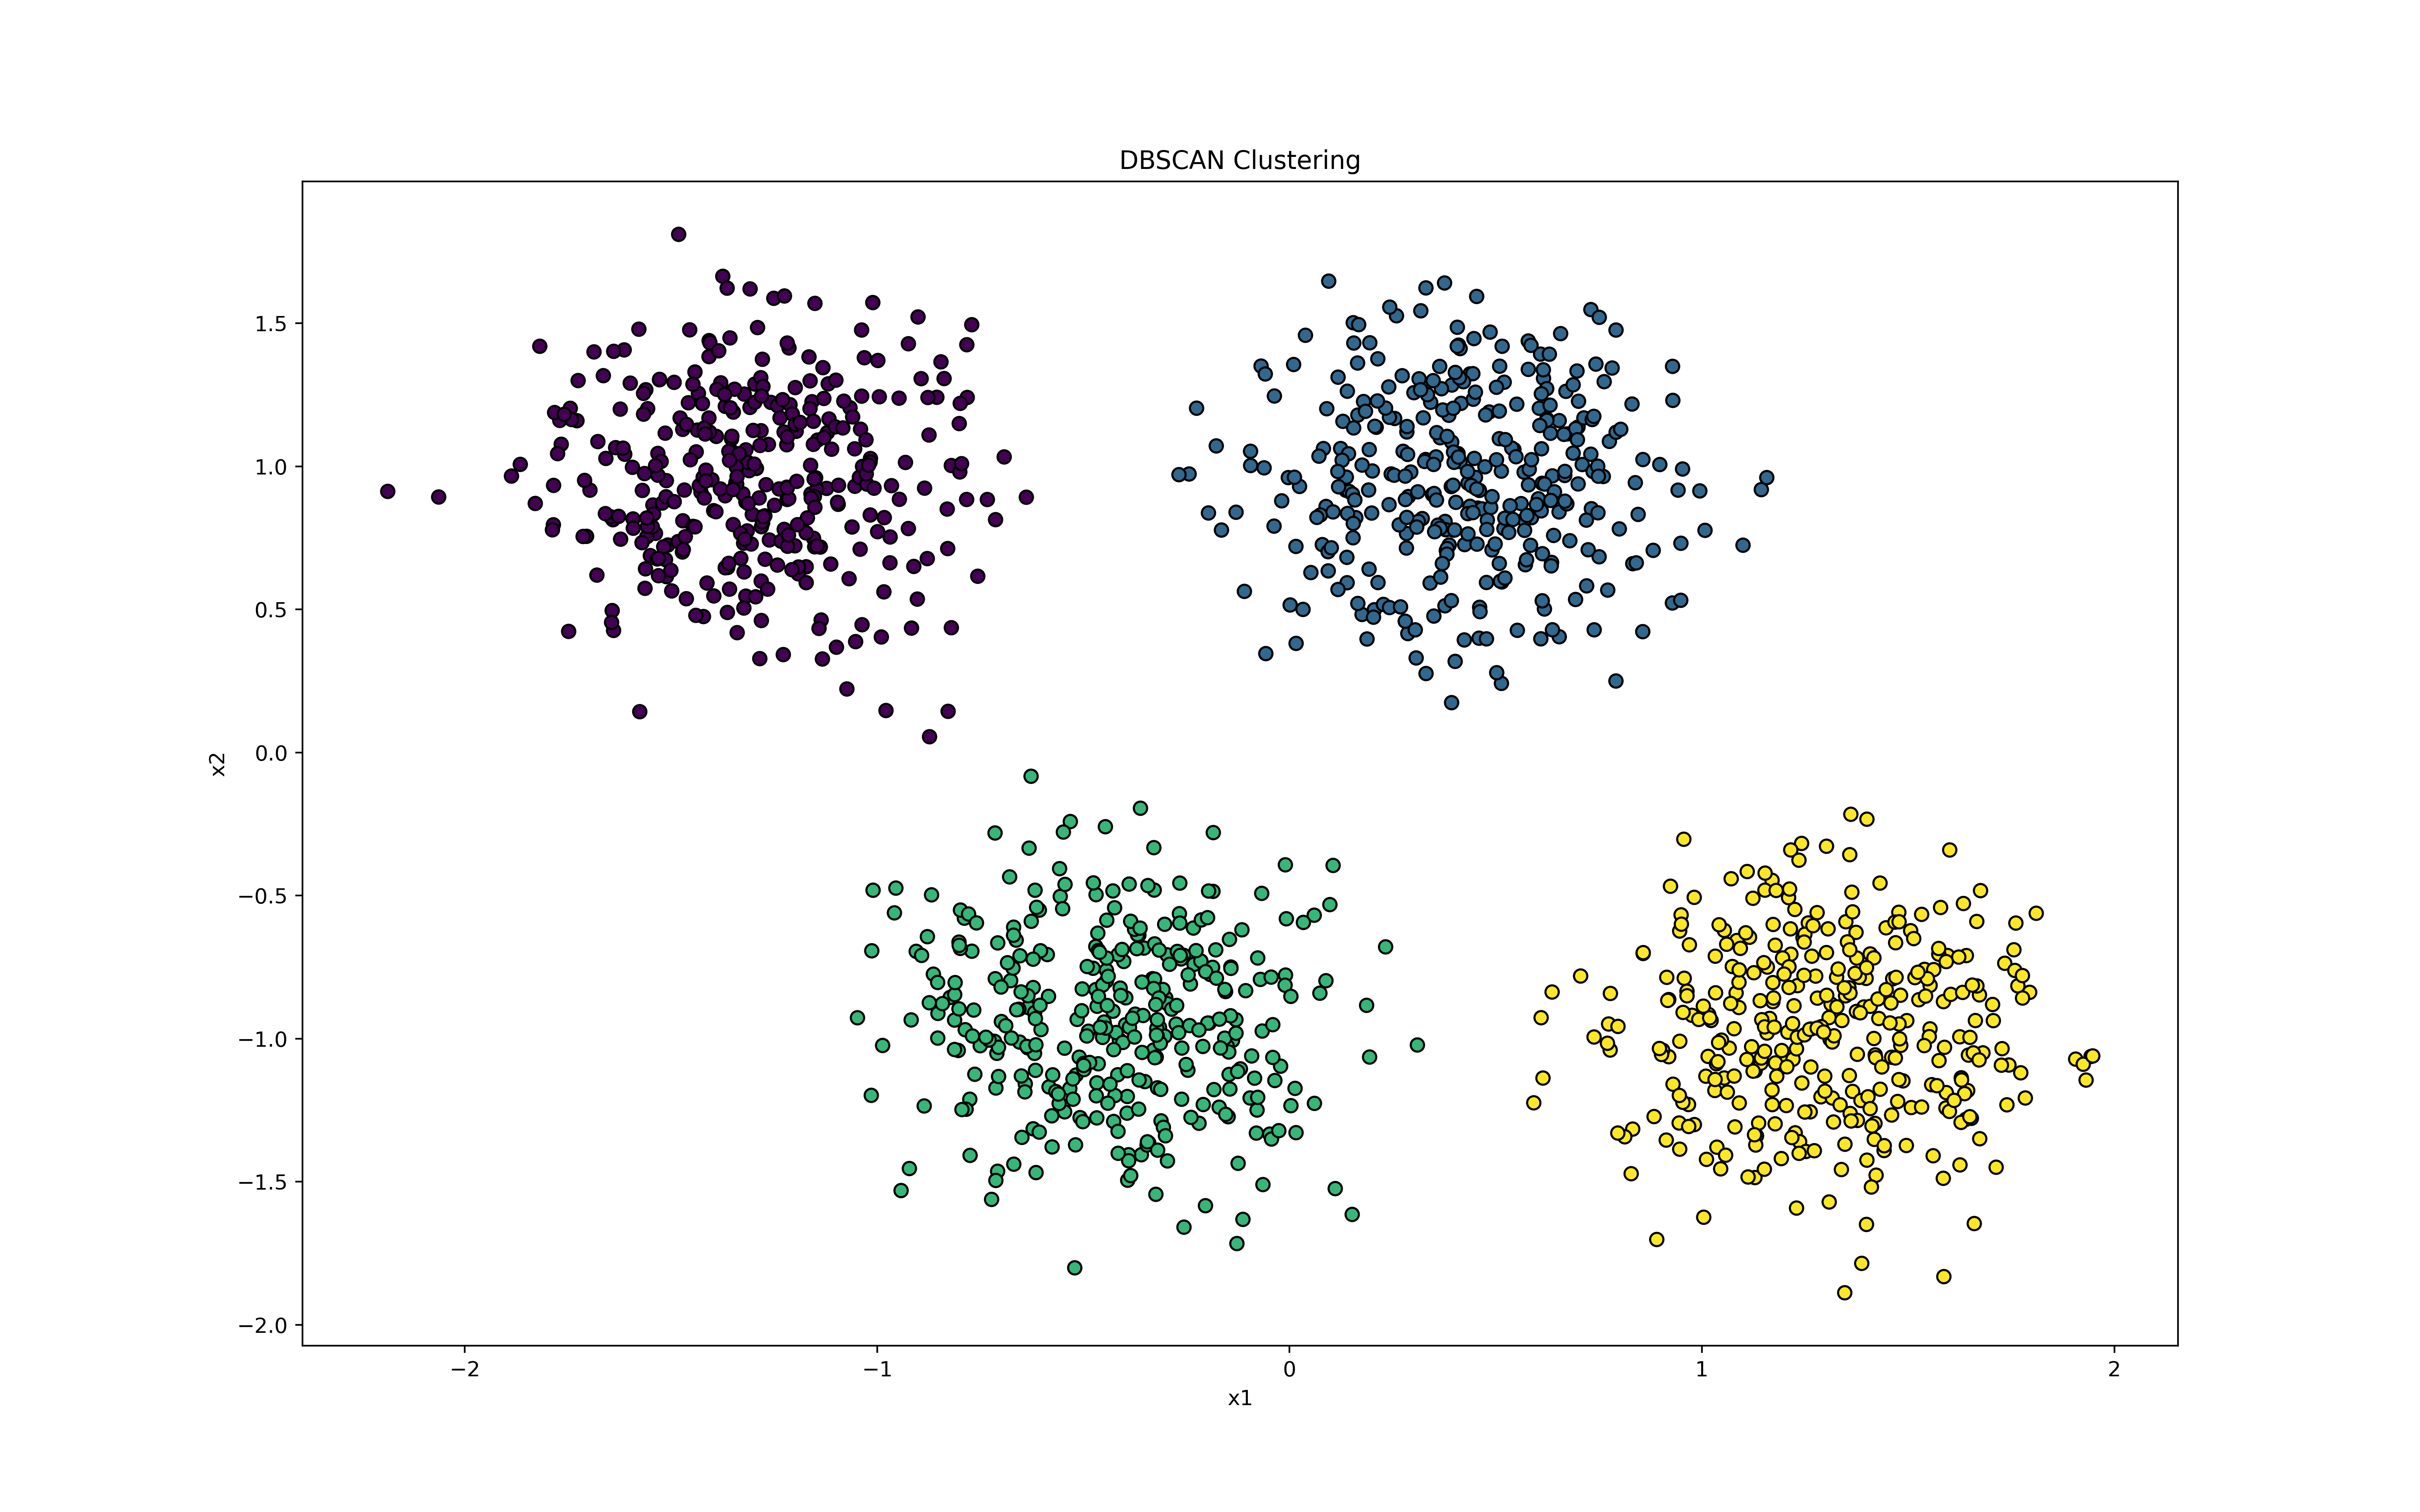
\includegraphics[width=0.75\linewidth]{Images/Clusters-5-v0-DBSCAN Clustering.png}
	\caption{Dataset 1: DBSCAN Clustering}
	\label{fig:clusters-5-v0-dbscan-clustering}
\end{figure}

All 3 algorithms give almost the same classification results, with the DBSCAN algorithm having the highest Silhouette Score. The DBSCAN algorithm has found the best parameters for the dataset, which is evident from the high Silhouette Score.

\clearpage

\begin{figure}[H]
	\centering
	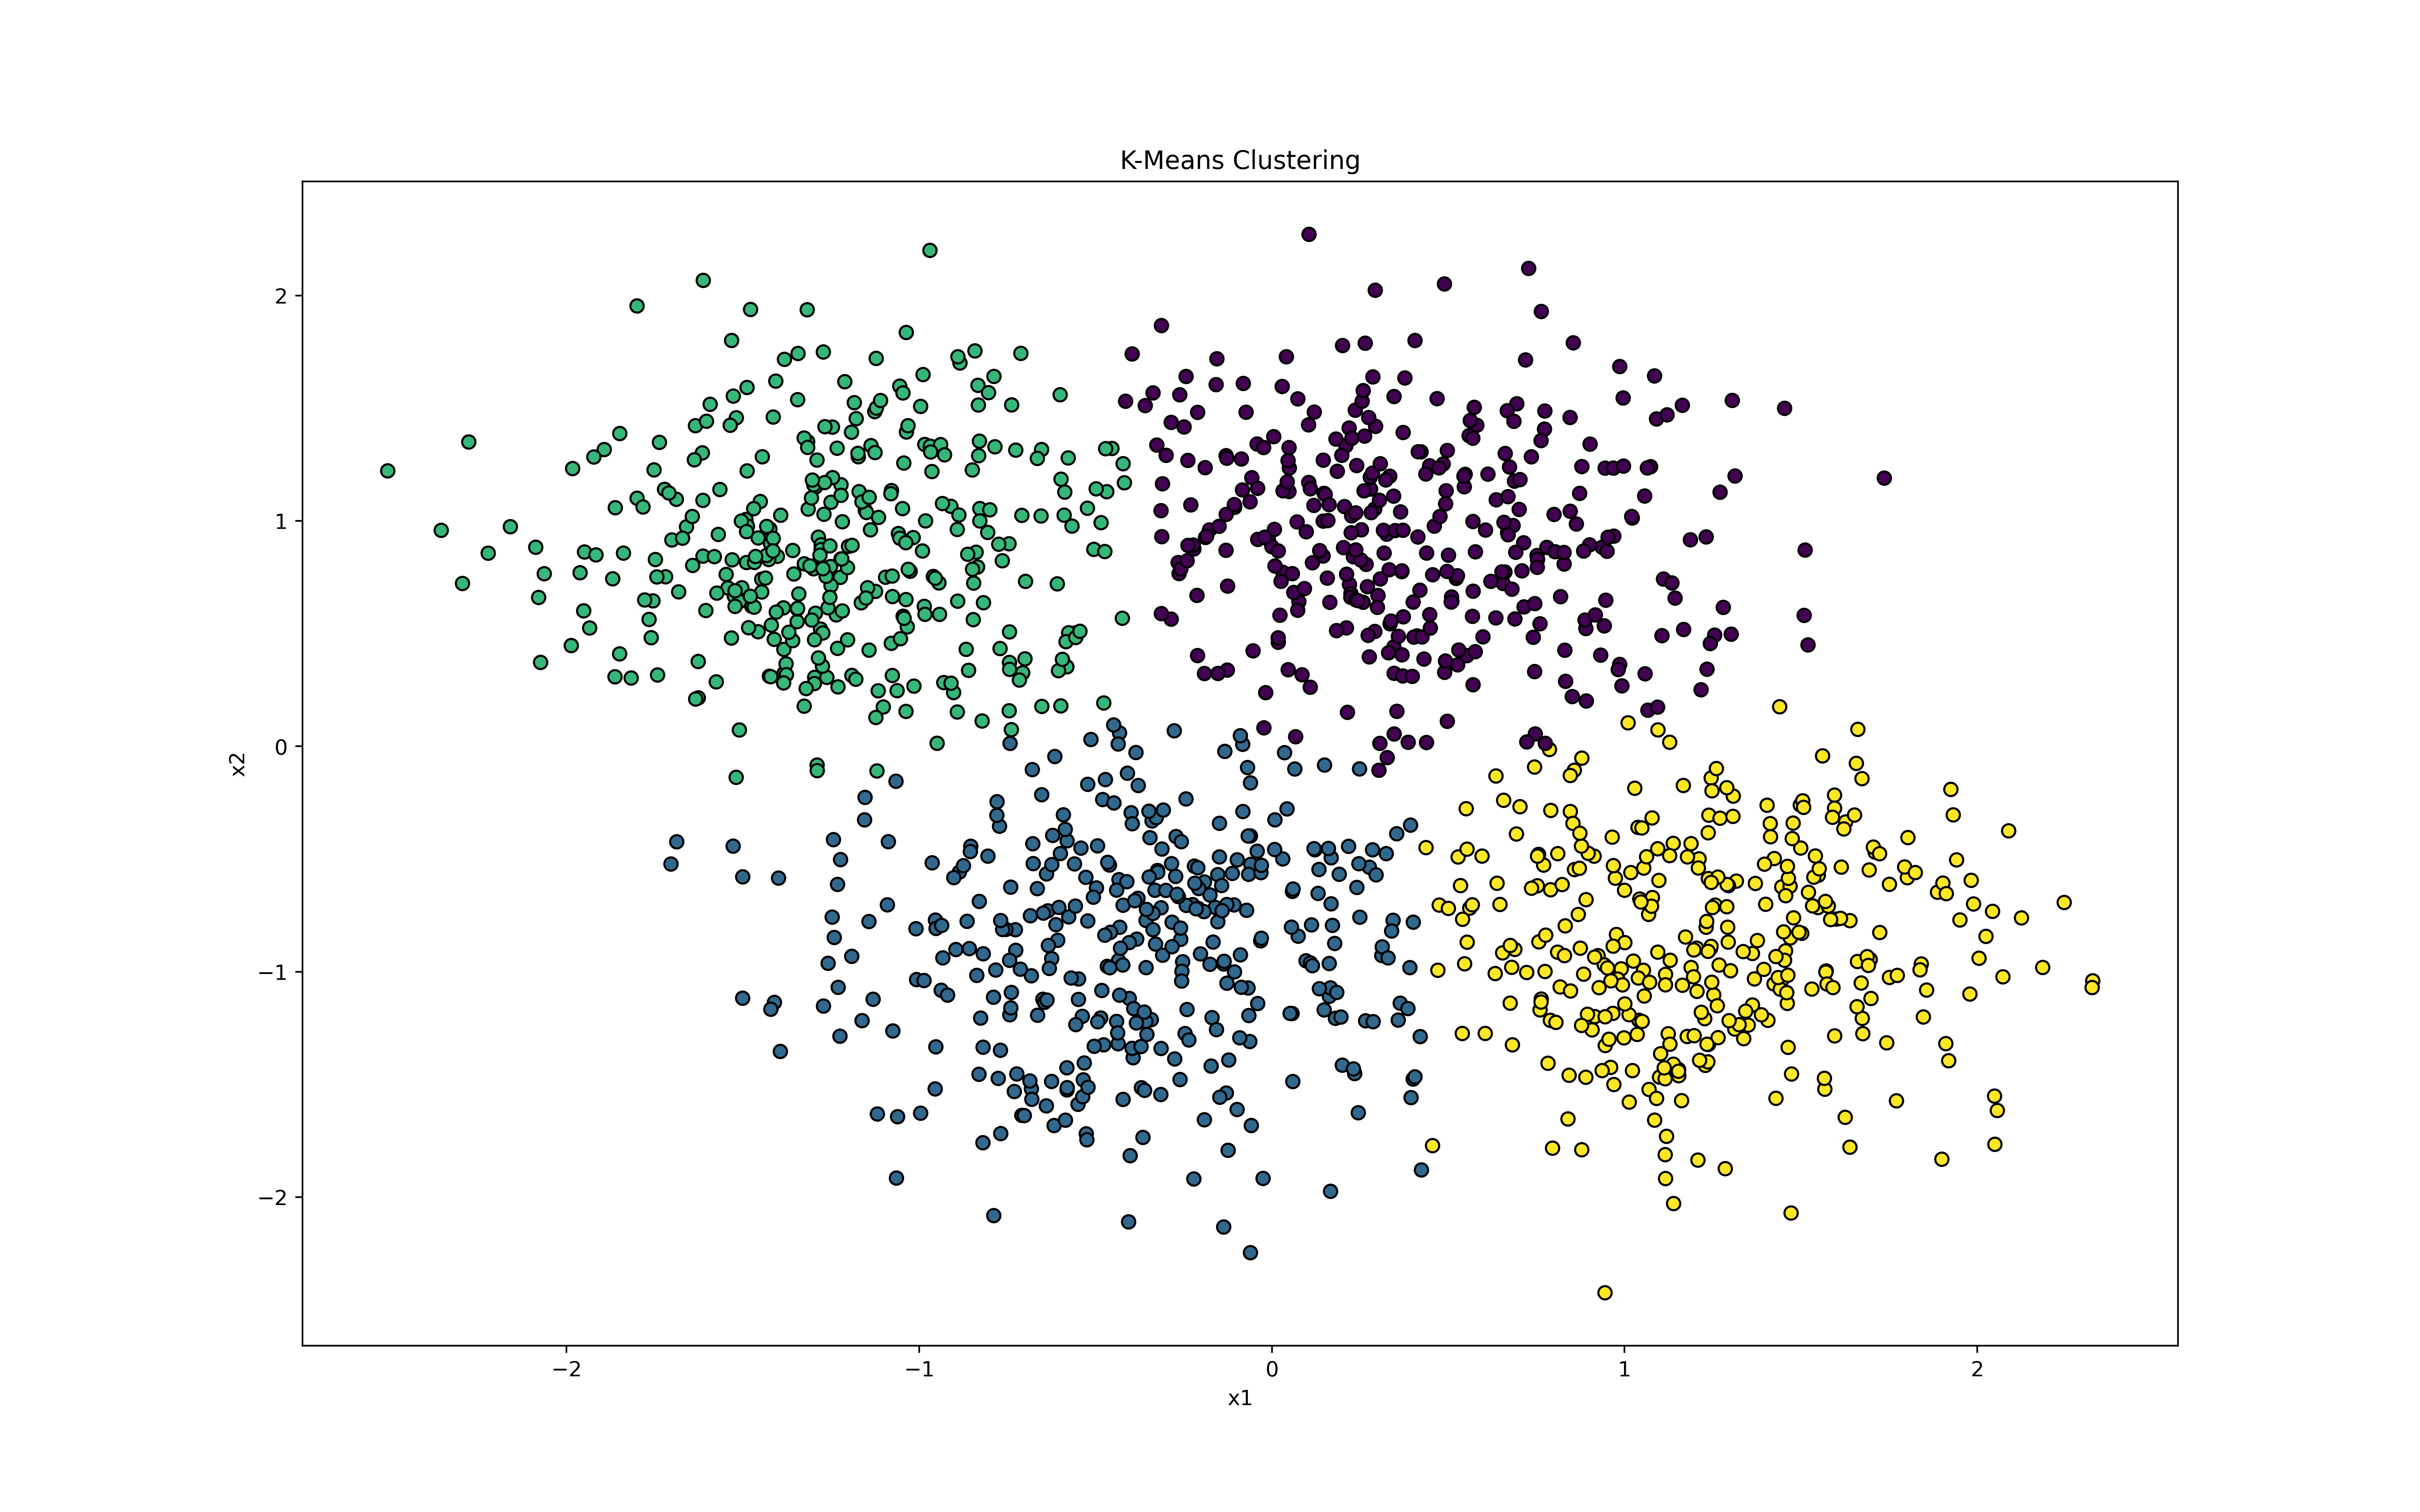
\includegraphics[width=0.9\linewidth]{Images/Clusters-5-v1-K-Means Clustering.png}
	\caption{Dataset 2: K-Means Clustering}
	\label{fig:clusters-5-v1-k-means-clustering}
\end{figure}

\begin{figure}[H]
	\centering
	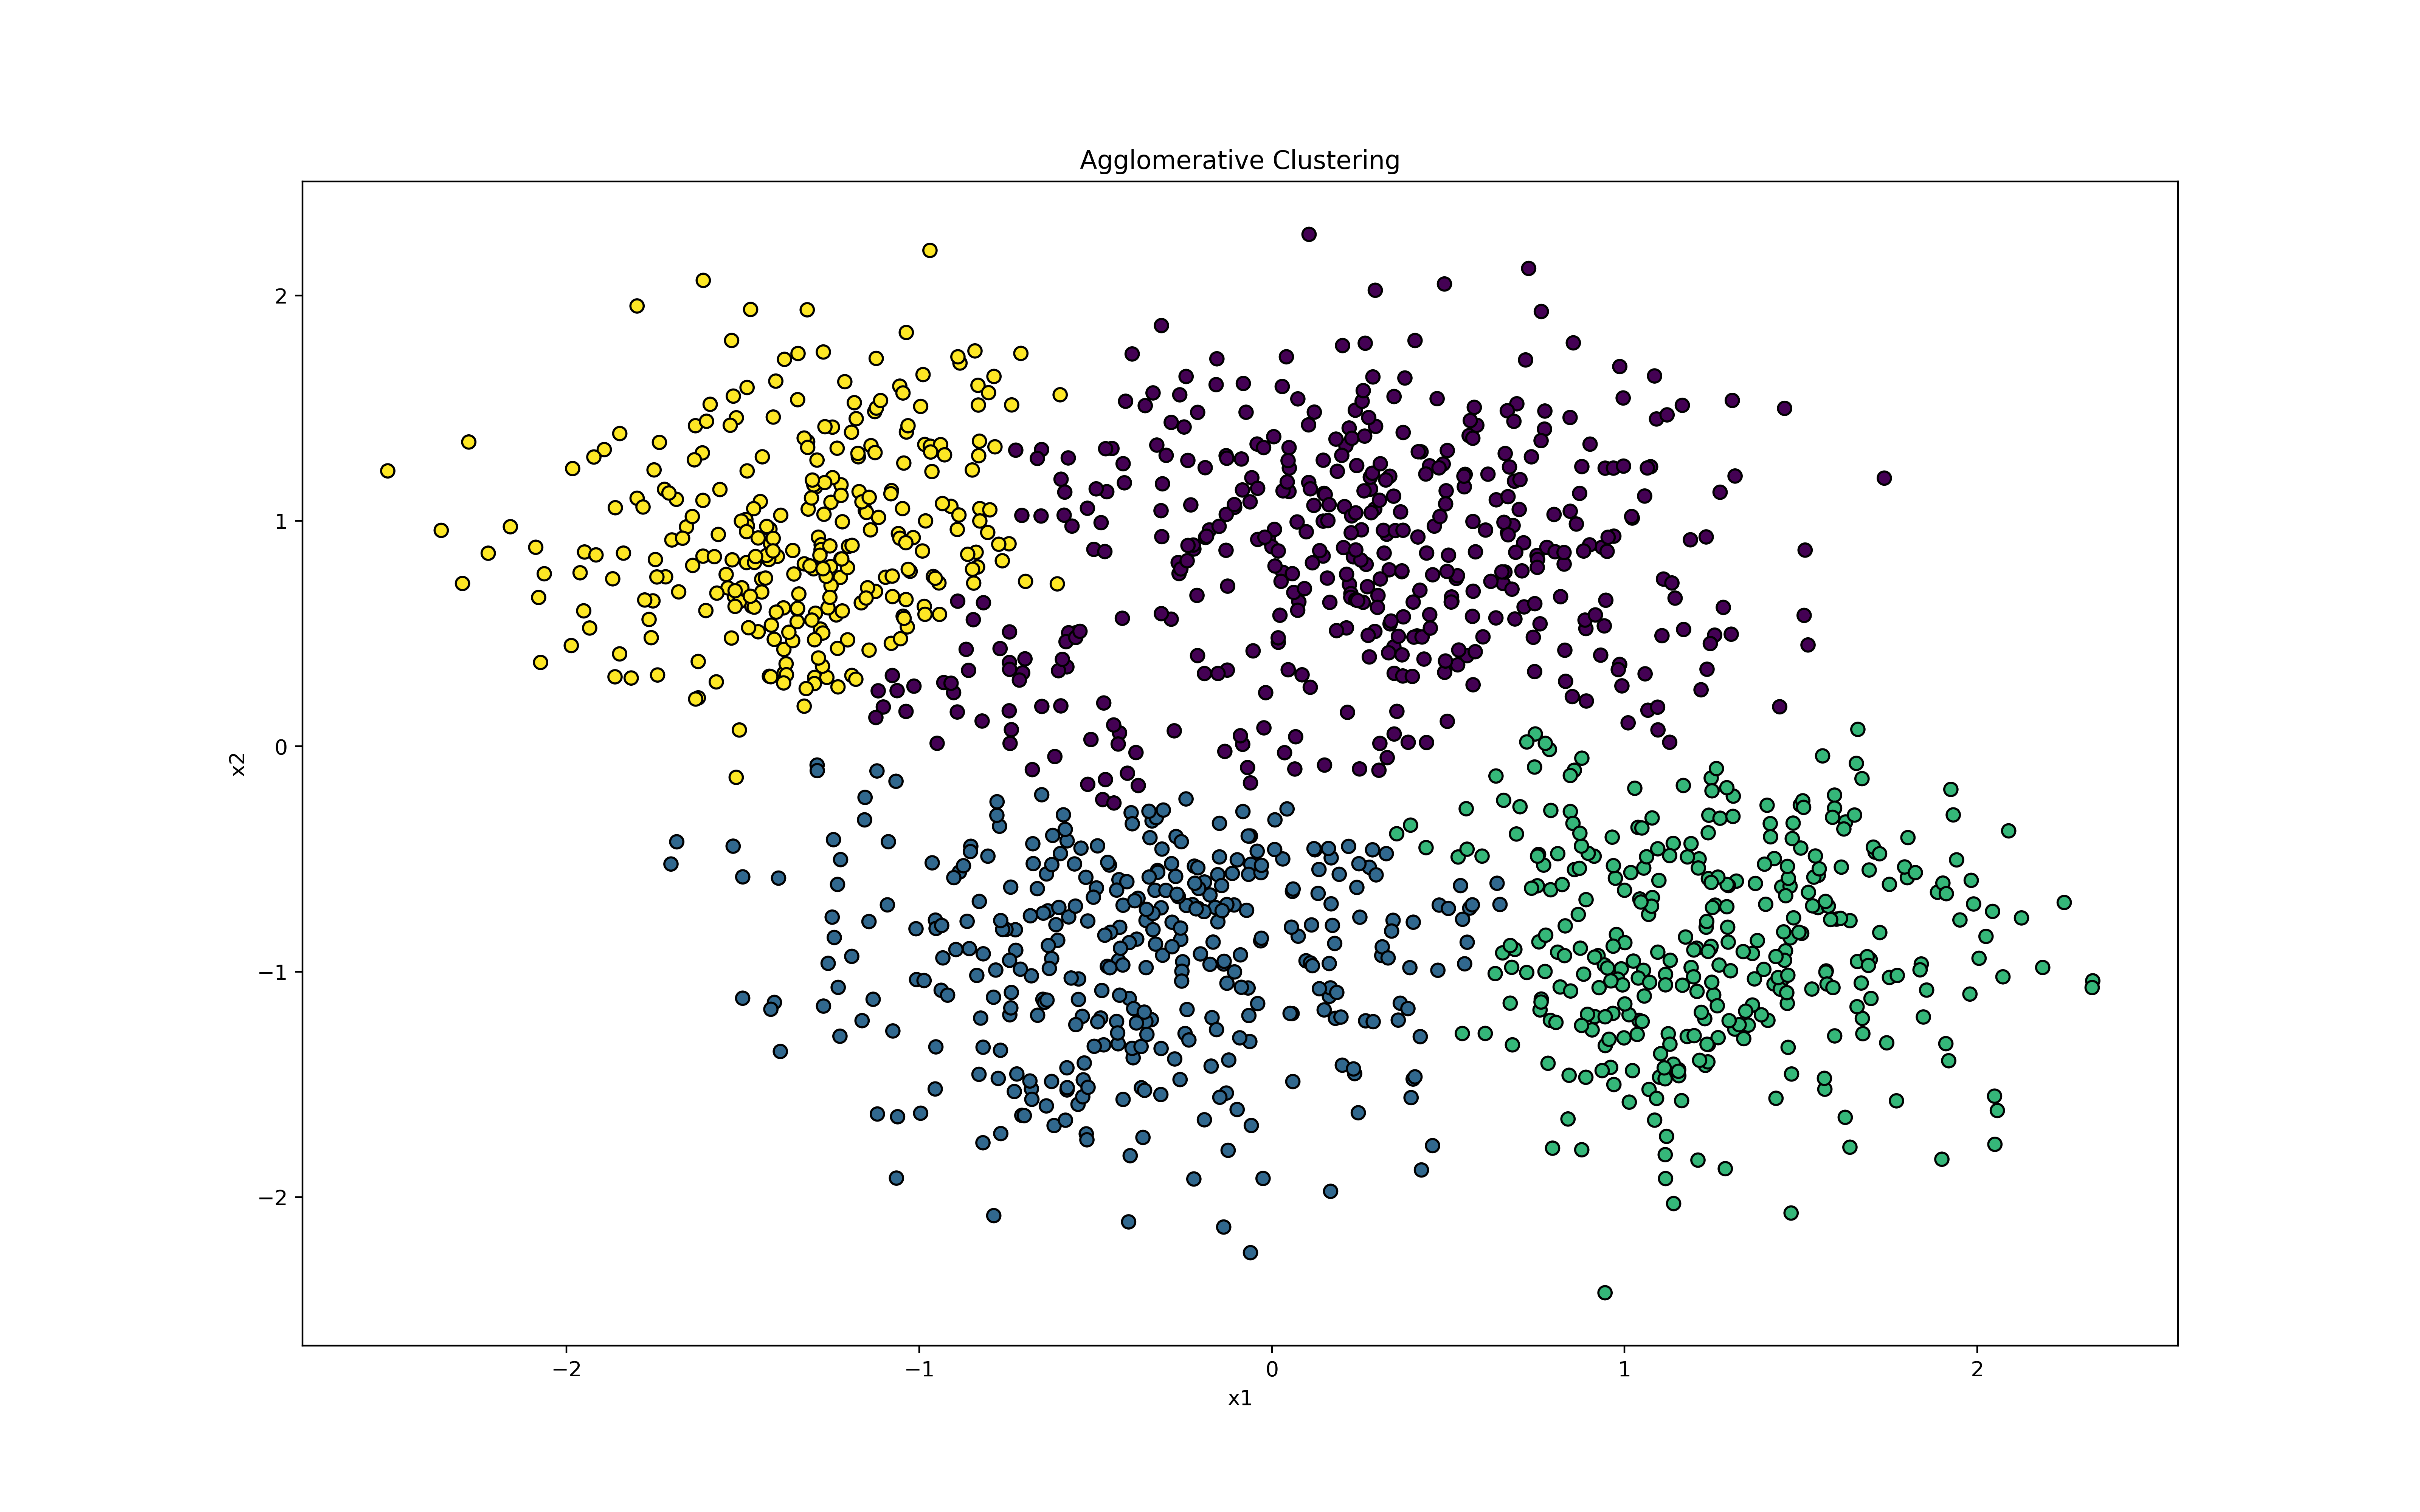
\includegraphics[width=0.9\linewidth]{Images/Clusters-5-v1-Agglomerative Clustering.png}
	\caption{Dataset 2: Agglomerative Clustering}
	\label{fig:clusters-5-v1-agglomerative-clustering}
\end{figure}

\begin{figure}[H]
    \centering
    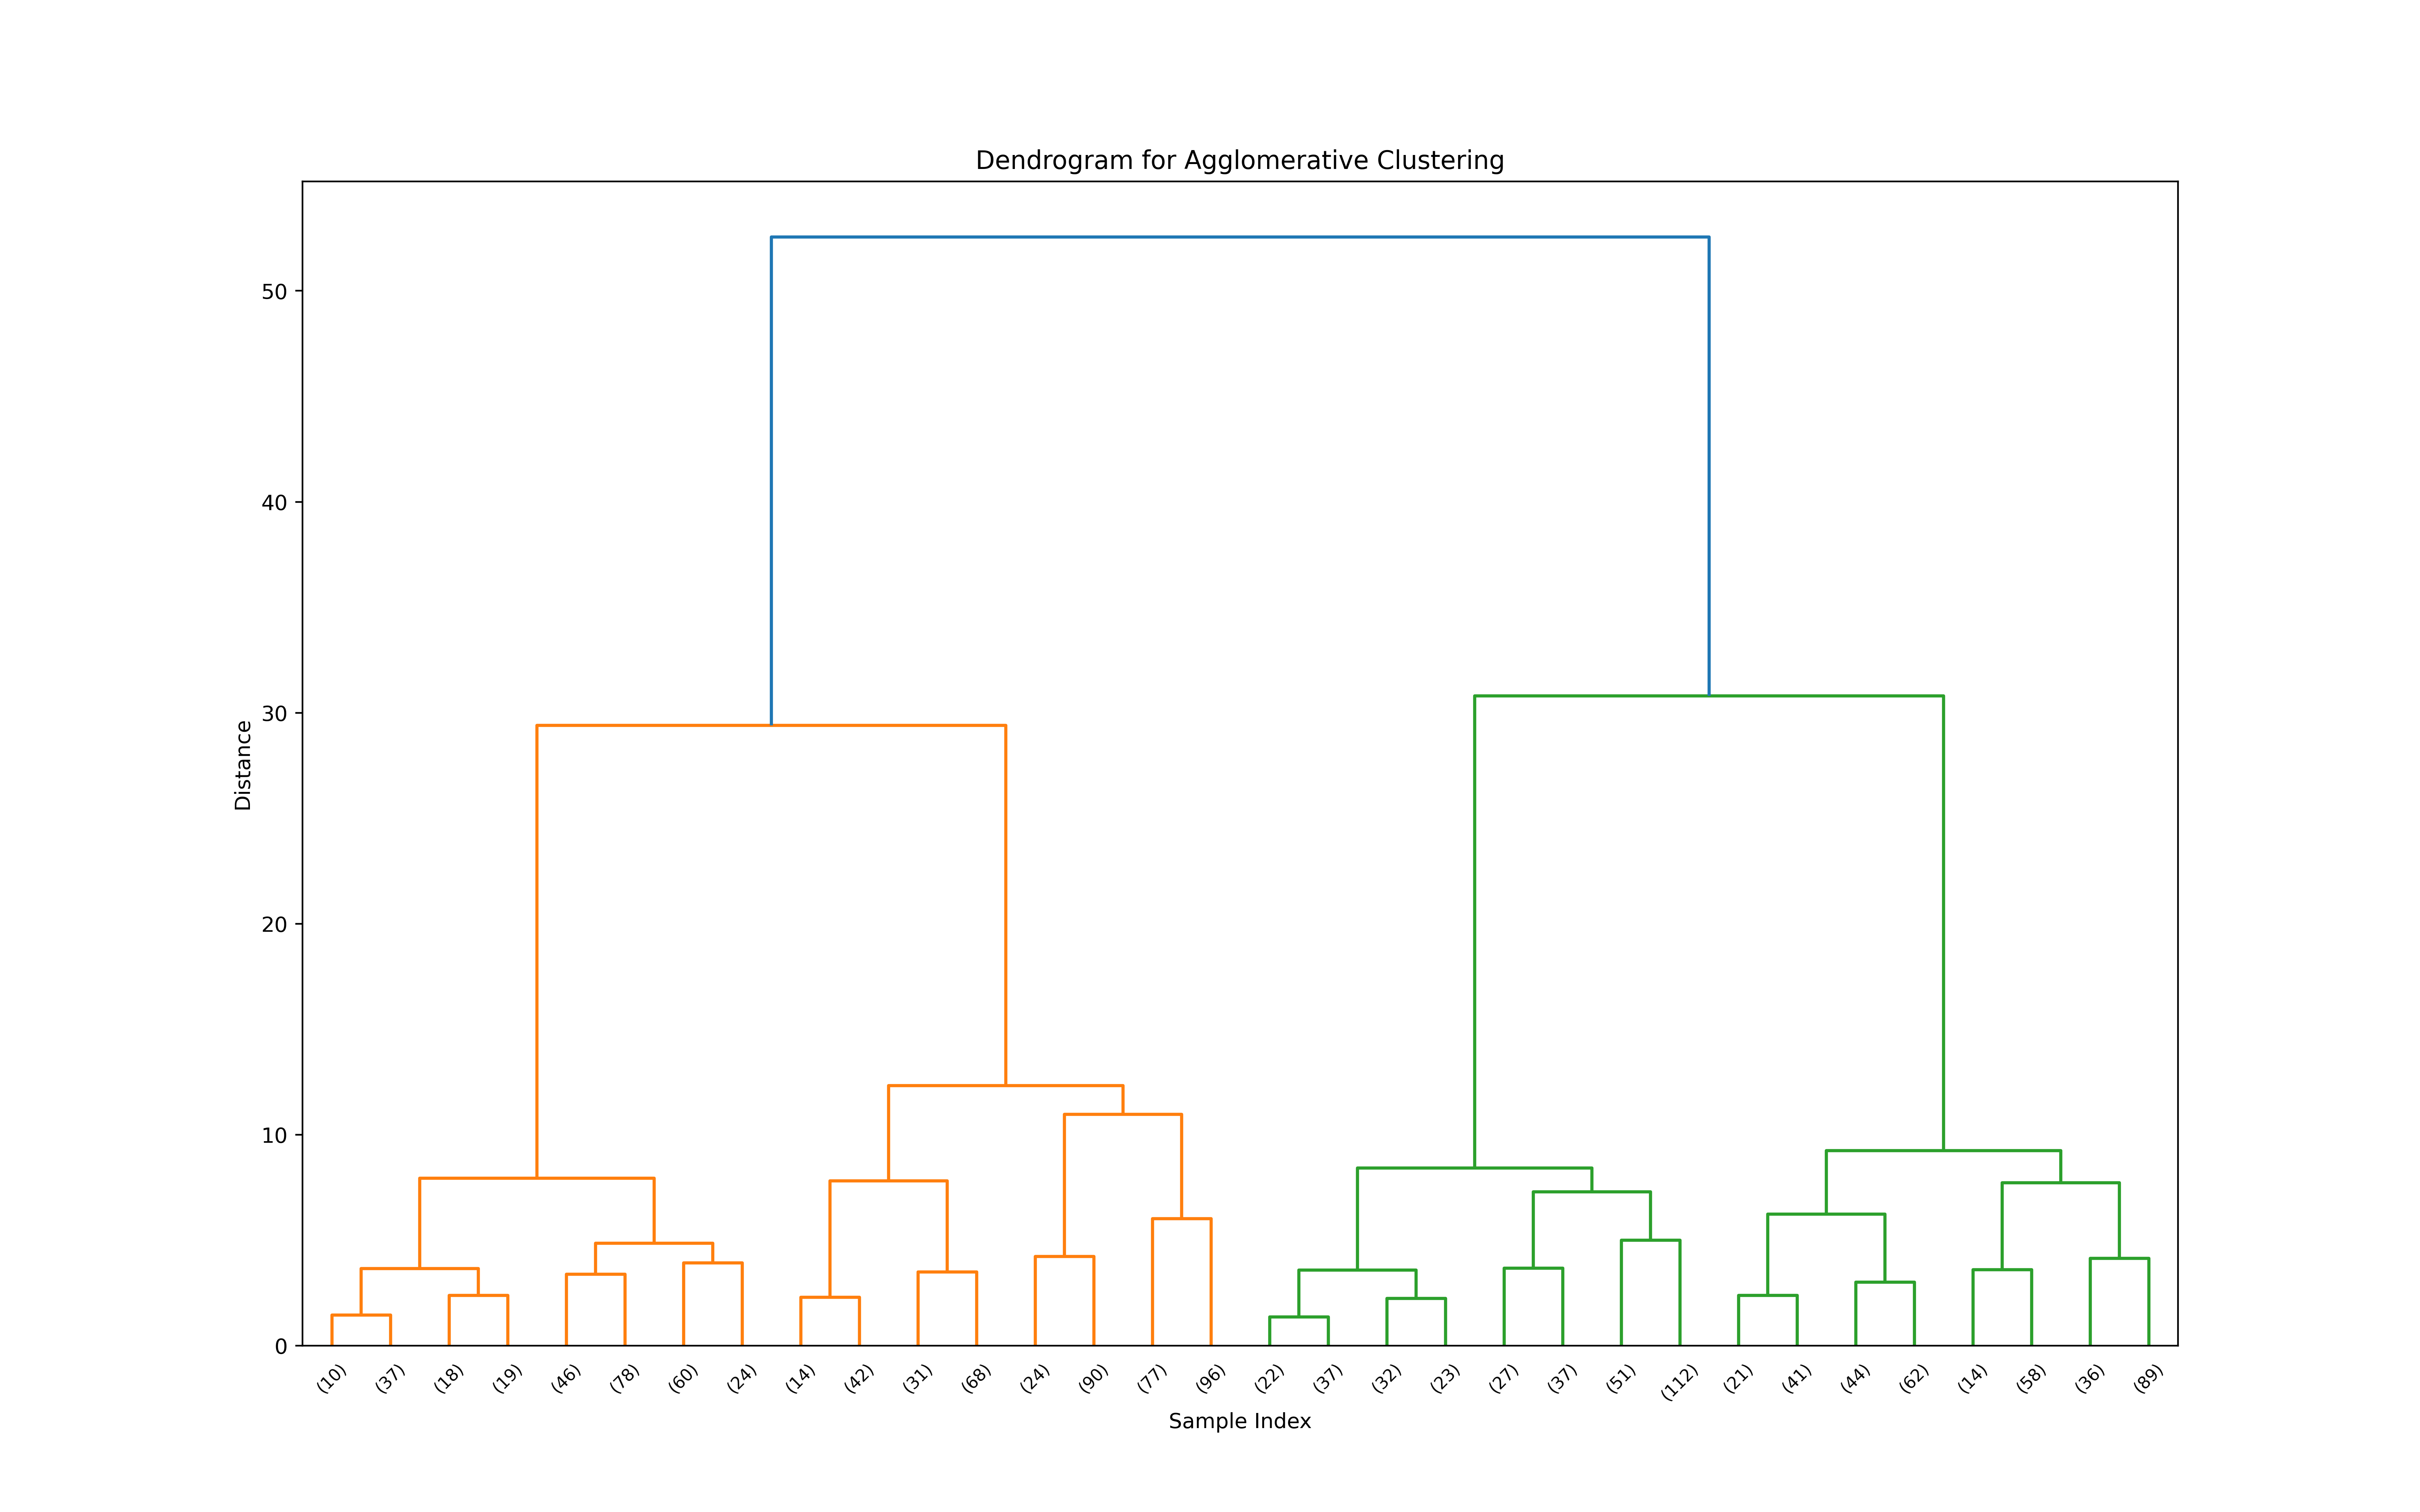
\includegraphics[width=0.75\linewidth]{Images/Clusters-5-v1-Agglomerative-Dendrogram.png}
    \caption{Dataset 2: Agglomerative Clustering Dendrogram}
    \label{fig:clusters-5-v1-agglomerative-dendrogram}
\end{figure}

\begin{figure}[H]
	\centering
	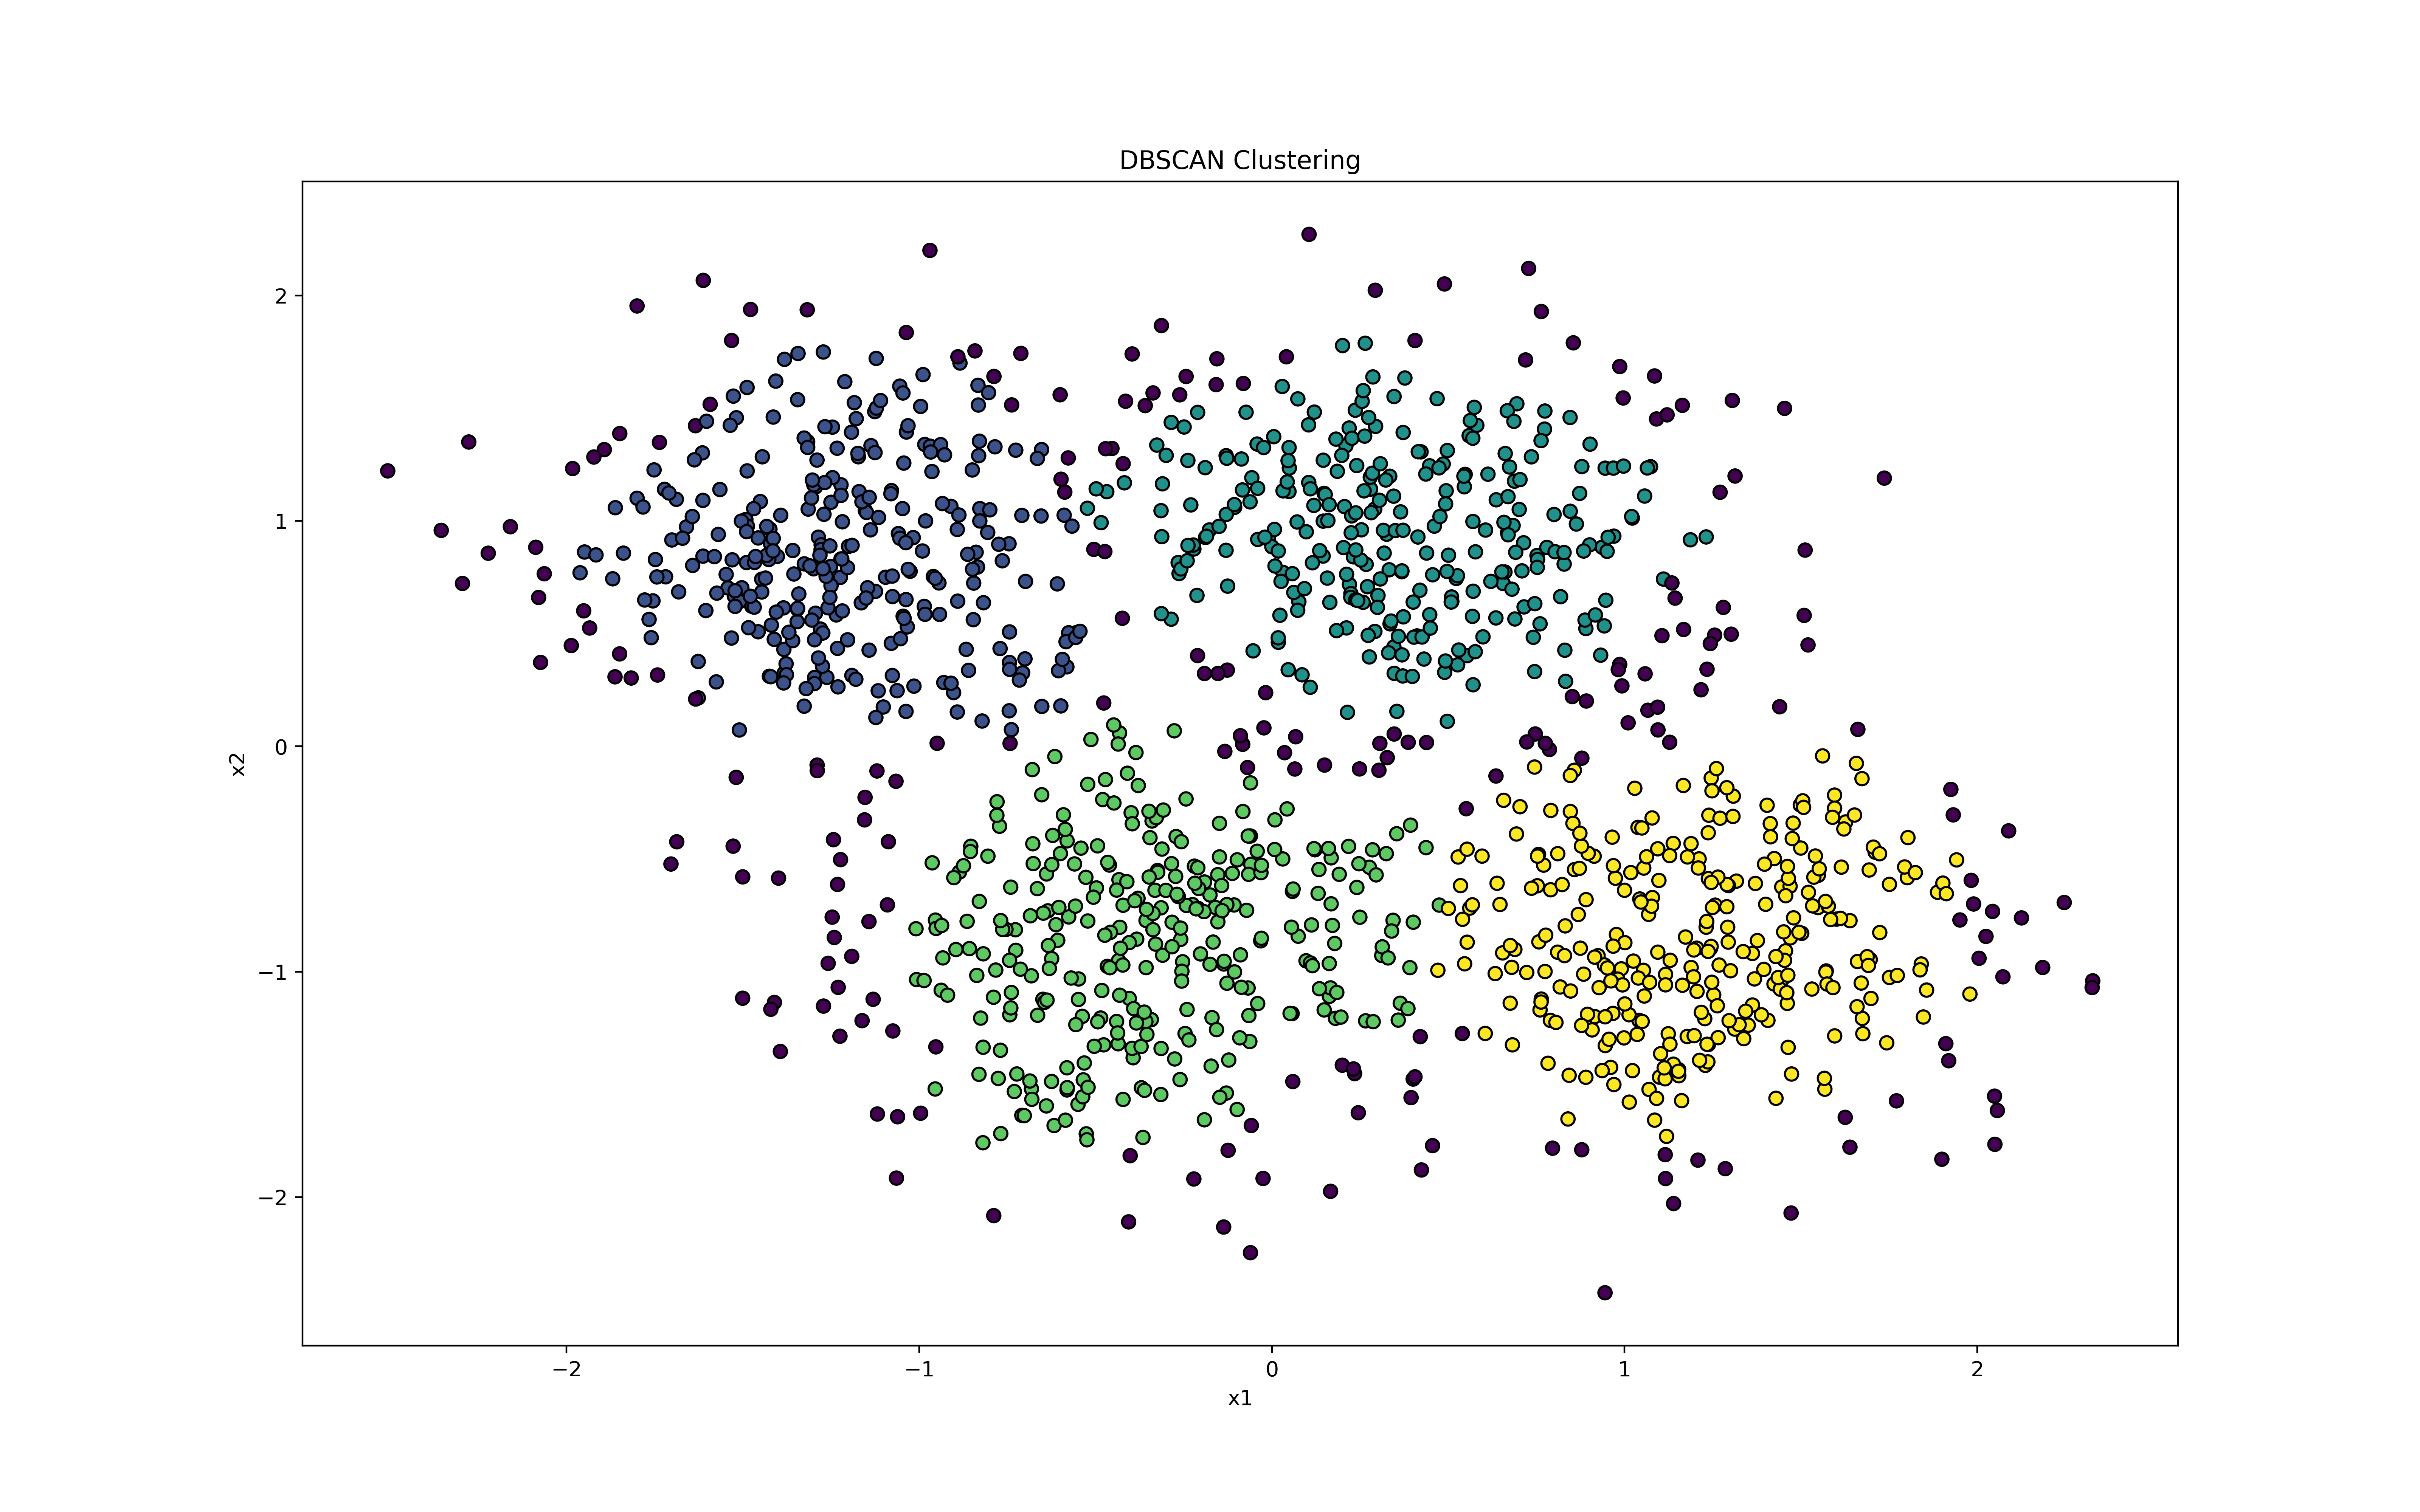
\includegraphics[width=0.75\linewidth]{Images/Clusters-5-v1-DBSCAN Clustering.png}
	\caption{Dataset 2: DBSCAN Clustering}
	\label{fig:clusters-5-v1-dbscan-clustering}
\end{figure}

We observe that K-Means and Agglomerative Clustering algorithms give satisfactory classifications for Dataset 2. The DBSCAN algorithm has not been able to find exactly 4 clusters for this dataset. \\

The Silhouette Score for DBSCAN is lower than that of K-Means and Agglomerative Clustering, indicating that the DBSCAN algorithm has not performed as well as the other two algorithms for this dataset.

\clearpage

\begin{figure}[H]
	\centering
	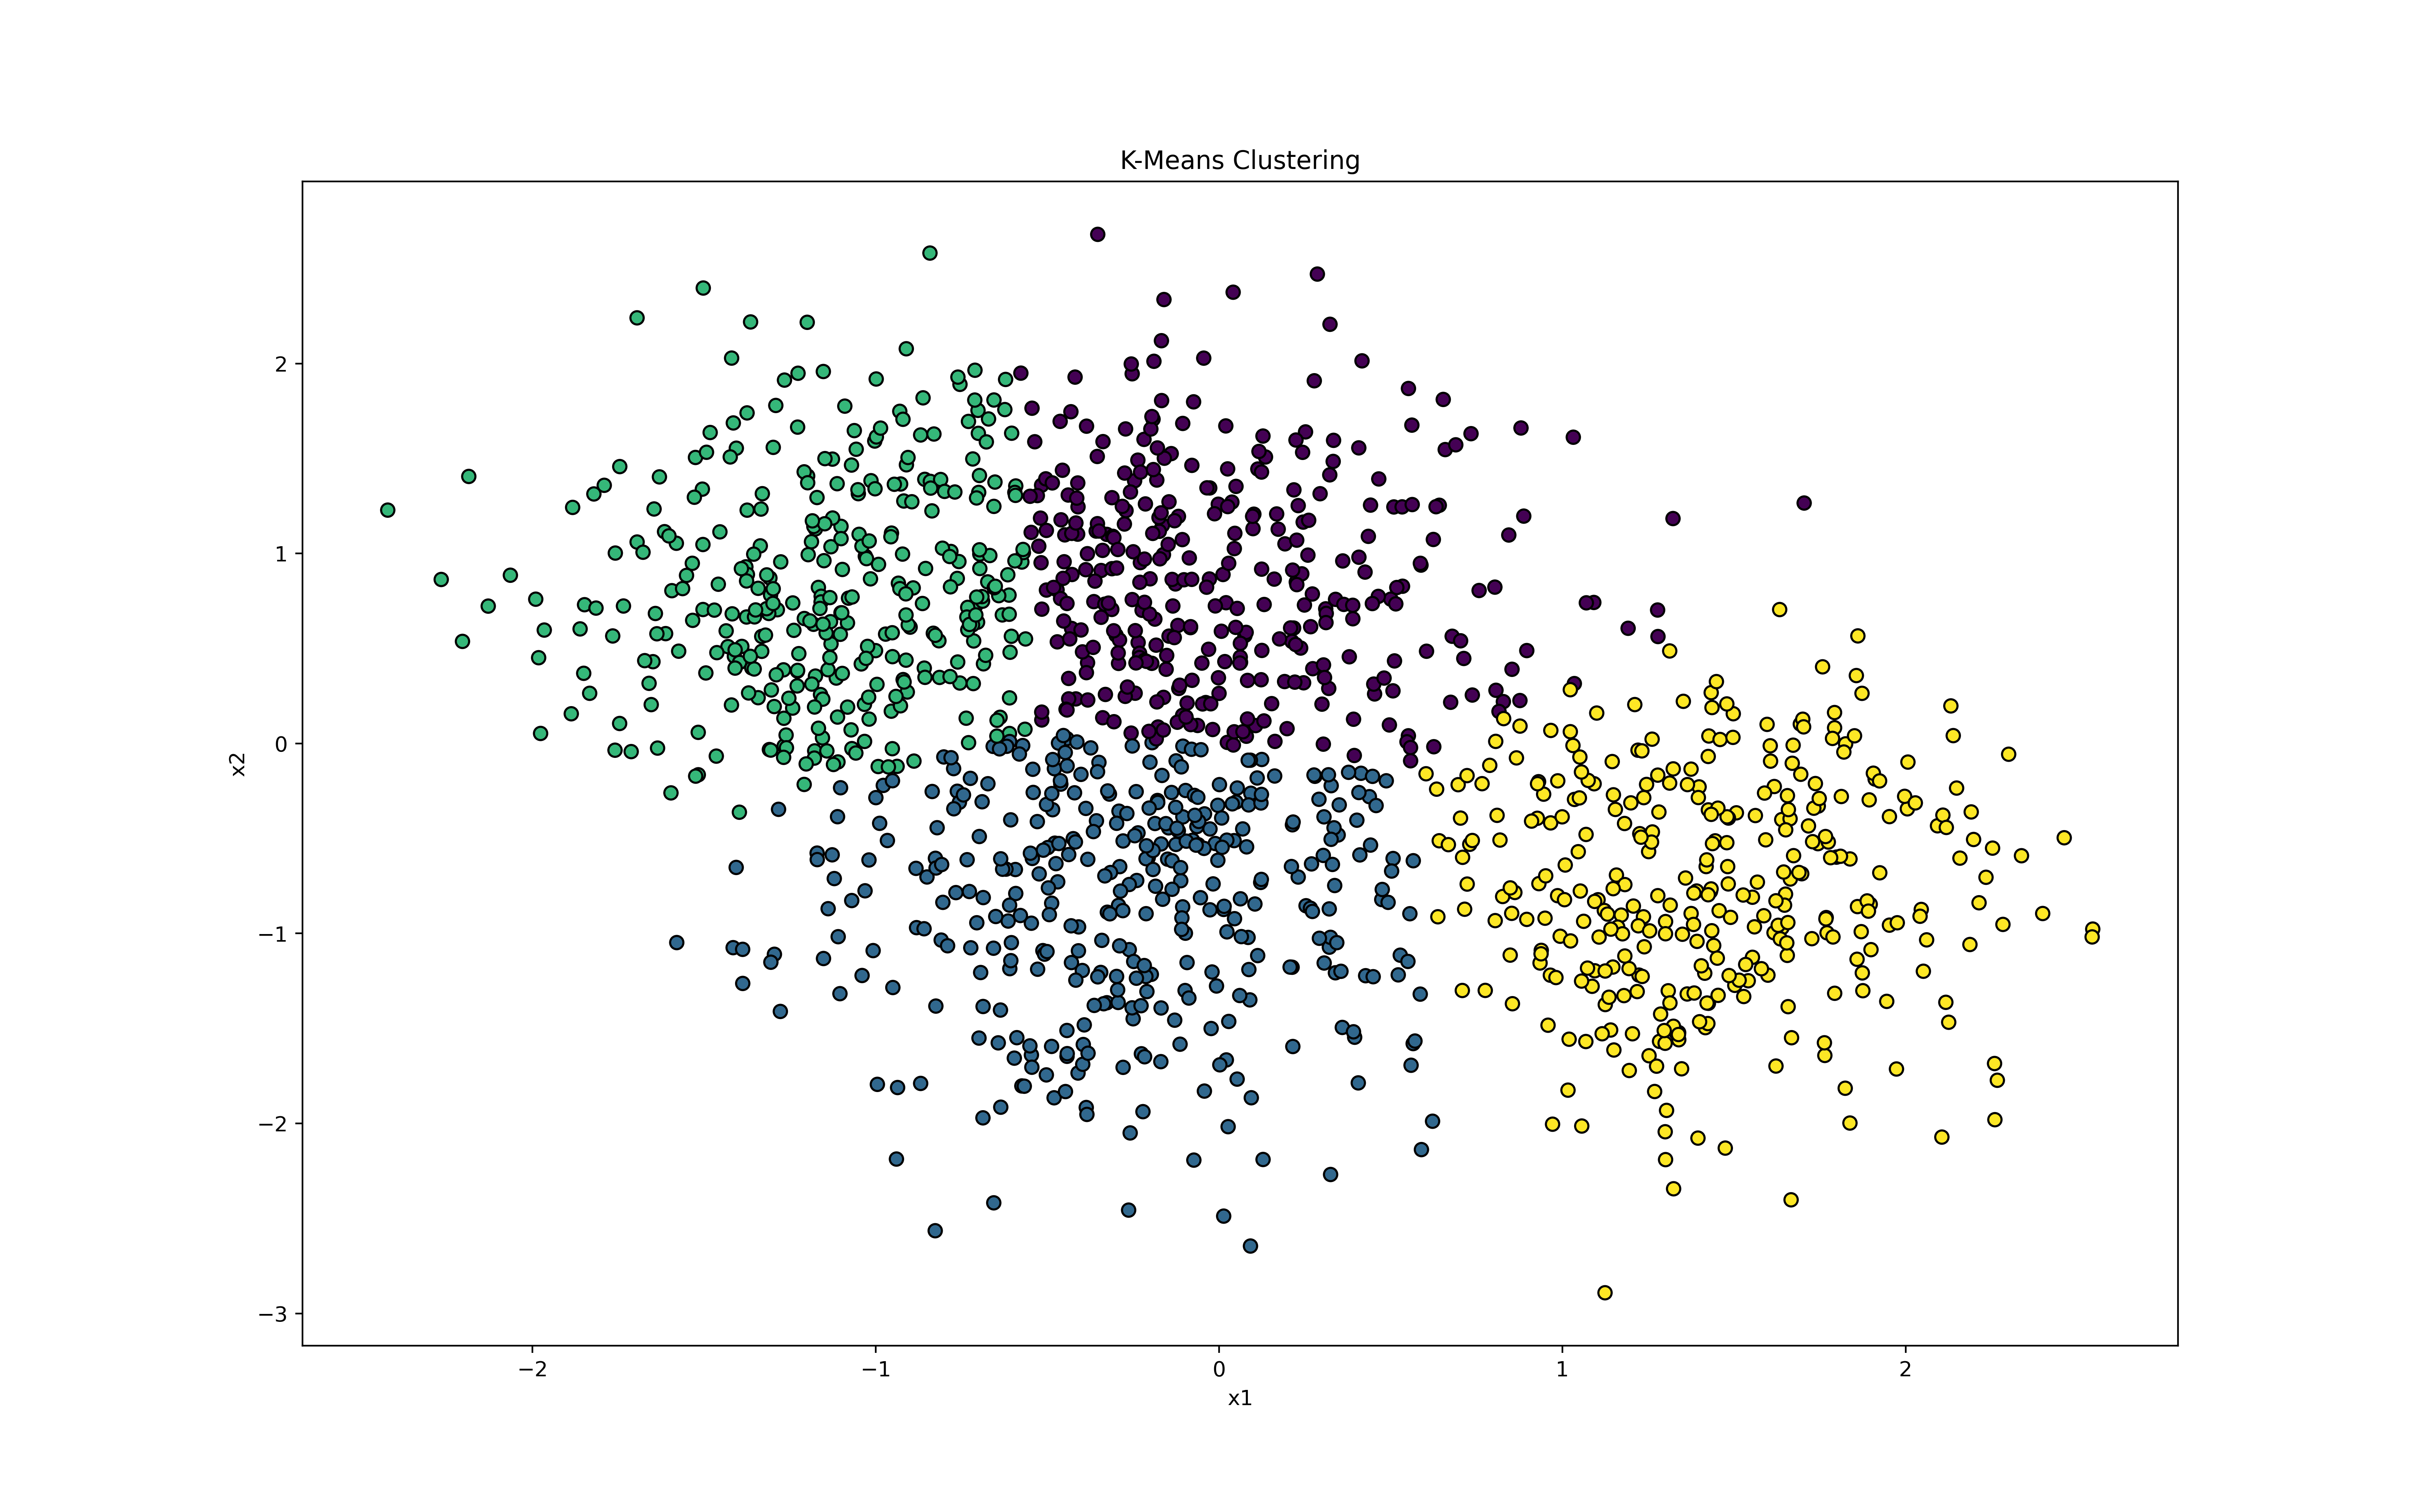
\includegraphics[width=0.9\linewidth]{Images/Clusters-5-v2-K-Means Clustering.png}
	\caption{Dataset 3: K-Means Clustering}
	\label{fig:clusters-5-v2-k-means-clustering}
\end{figure}

\begin{figure}[H]
	\centering
	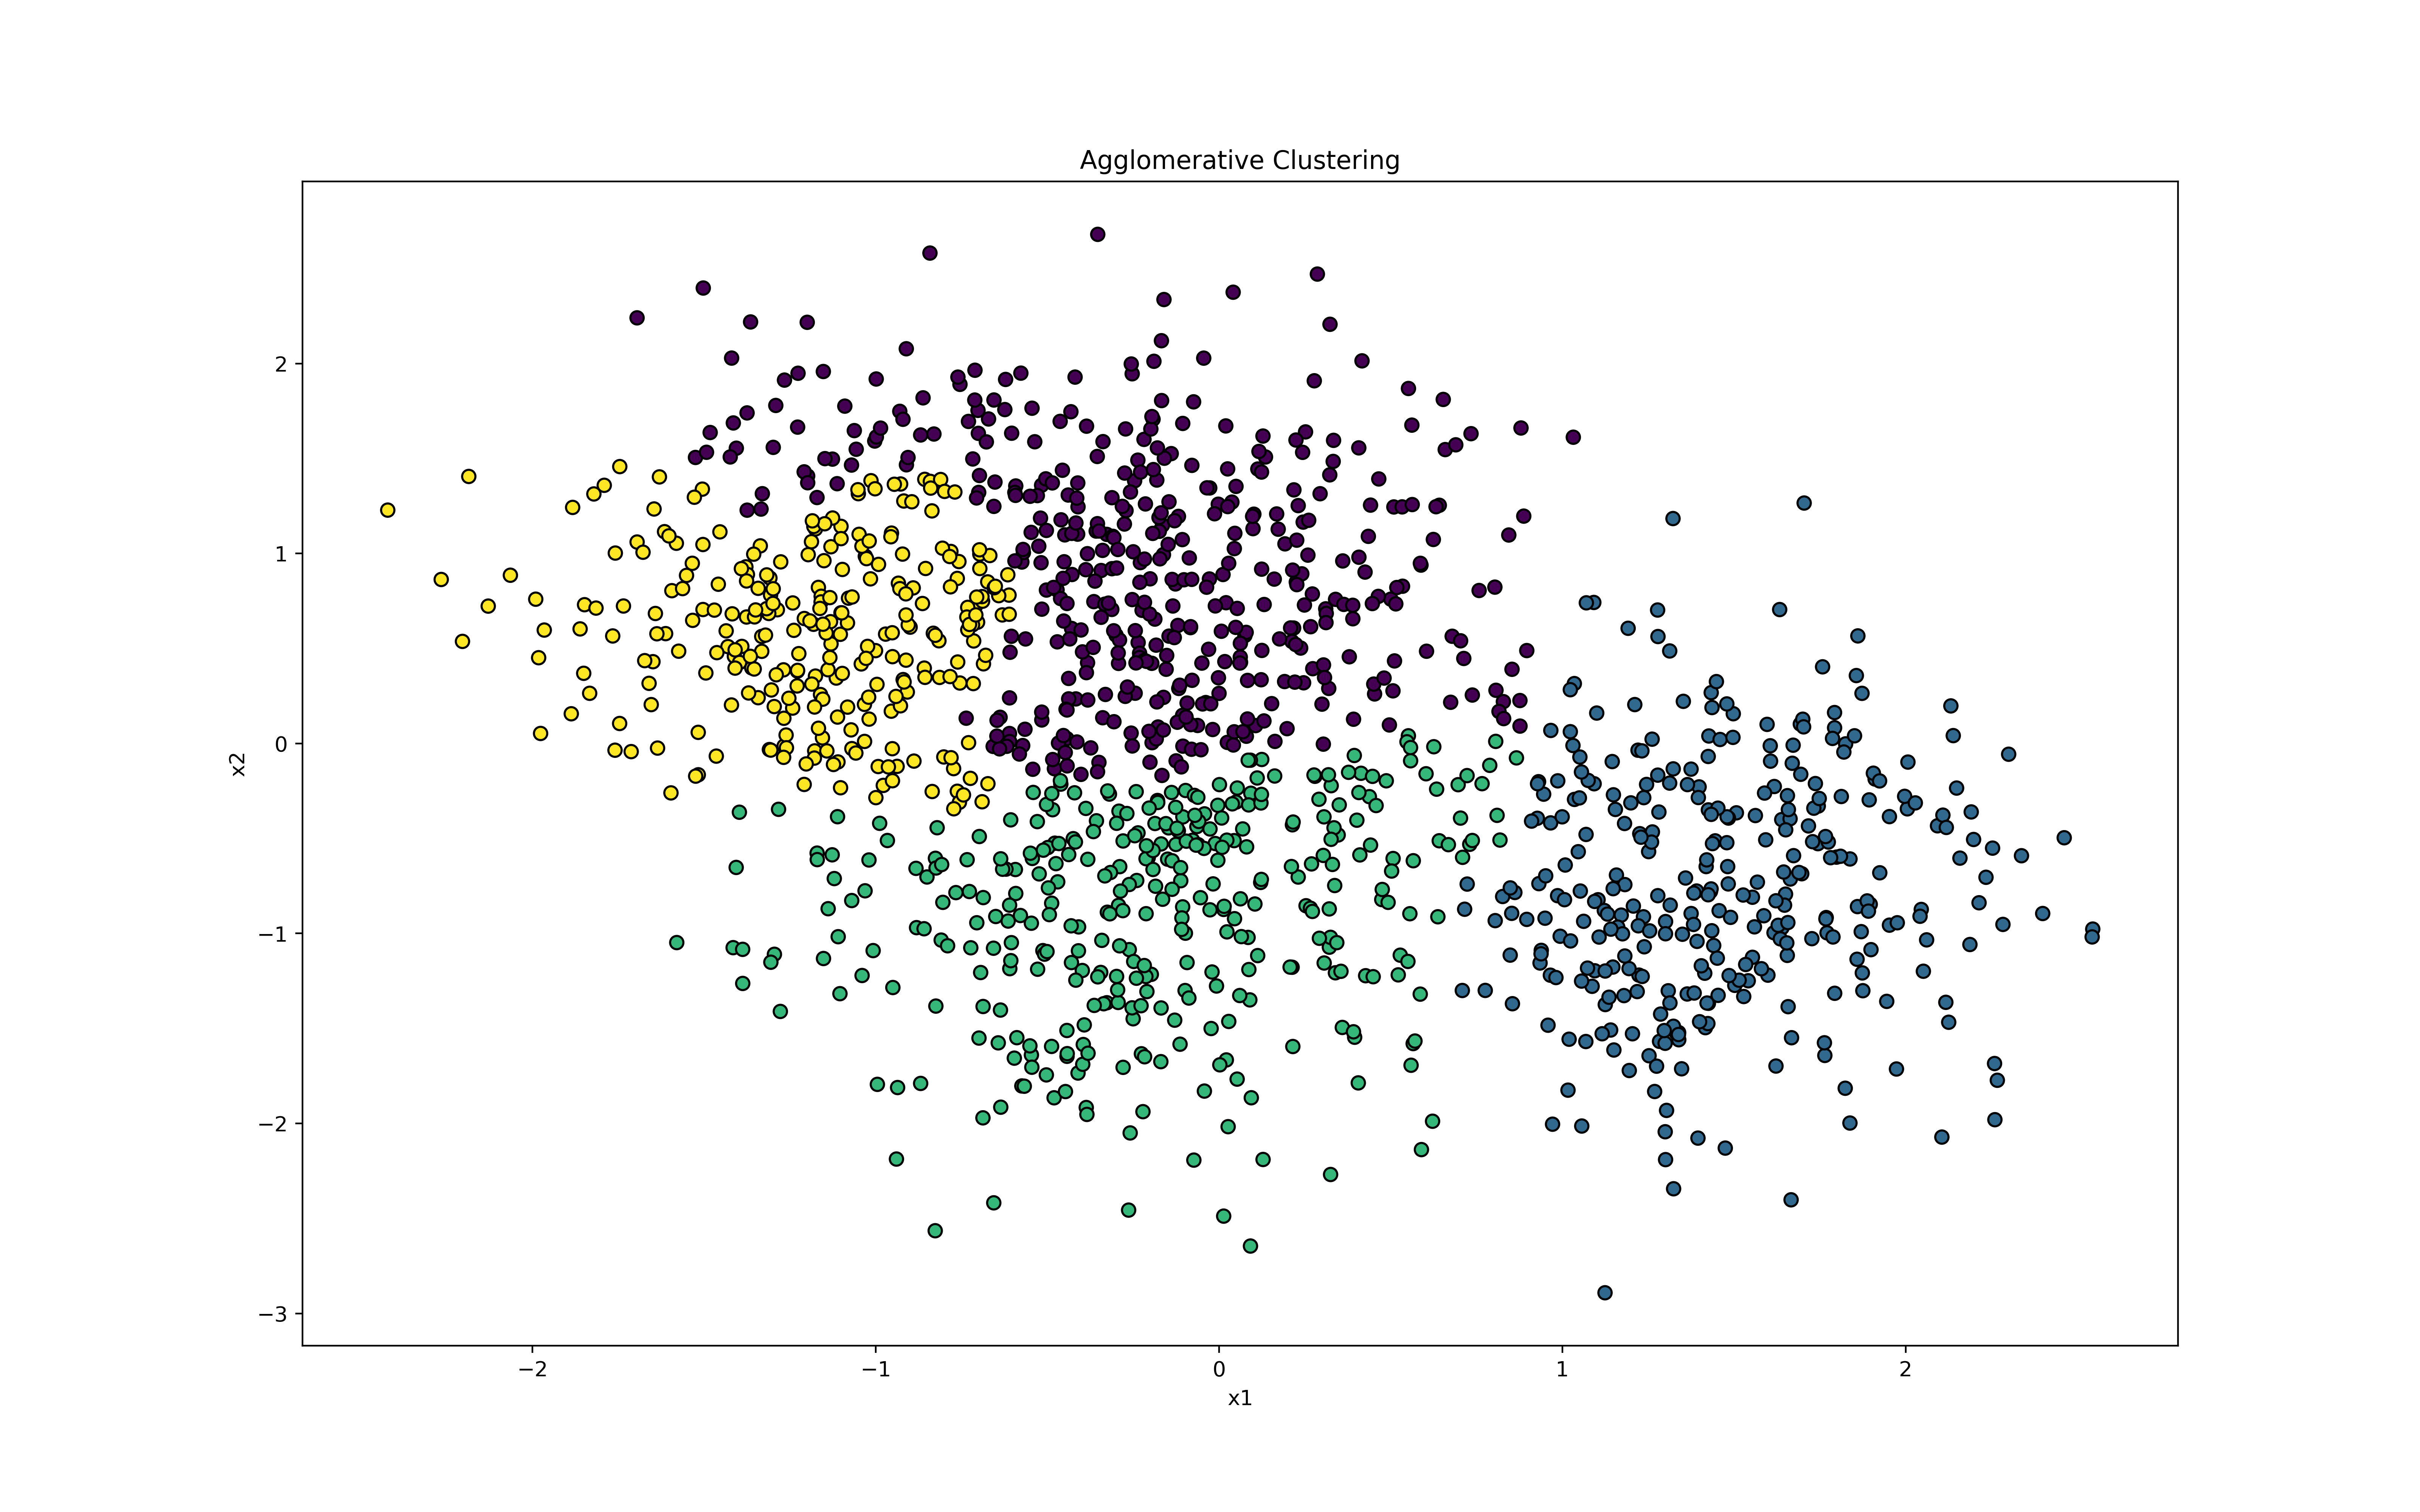
\includegraphics[width=0.9\linewidth]{Images/Clusters-5-v2-Agglomerative Clustering.png}
	\caption{Dataset 3: Agglomerative Clustering}
	\label{fig:clusters-5-v2-agglomerative-clustering}
\end{figure}

\begin{figure}[H]
    \centering
    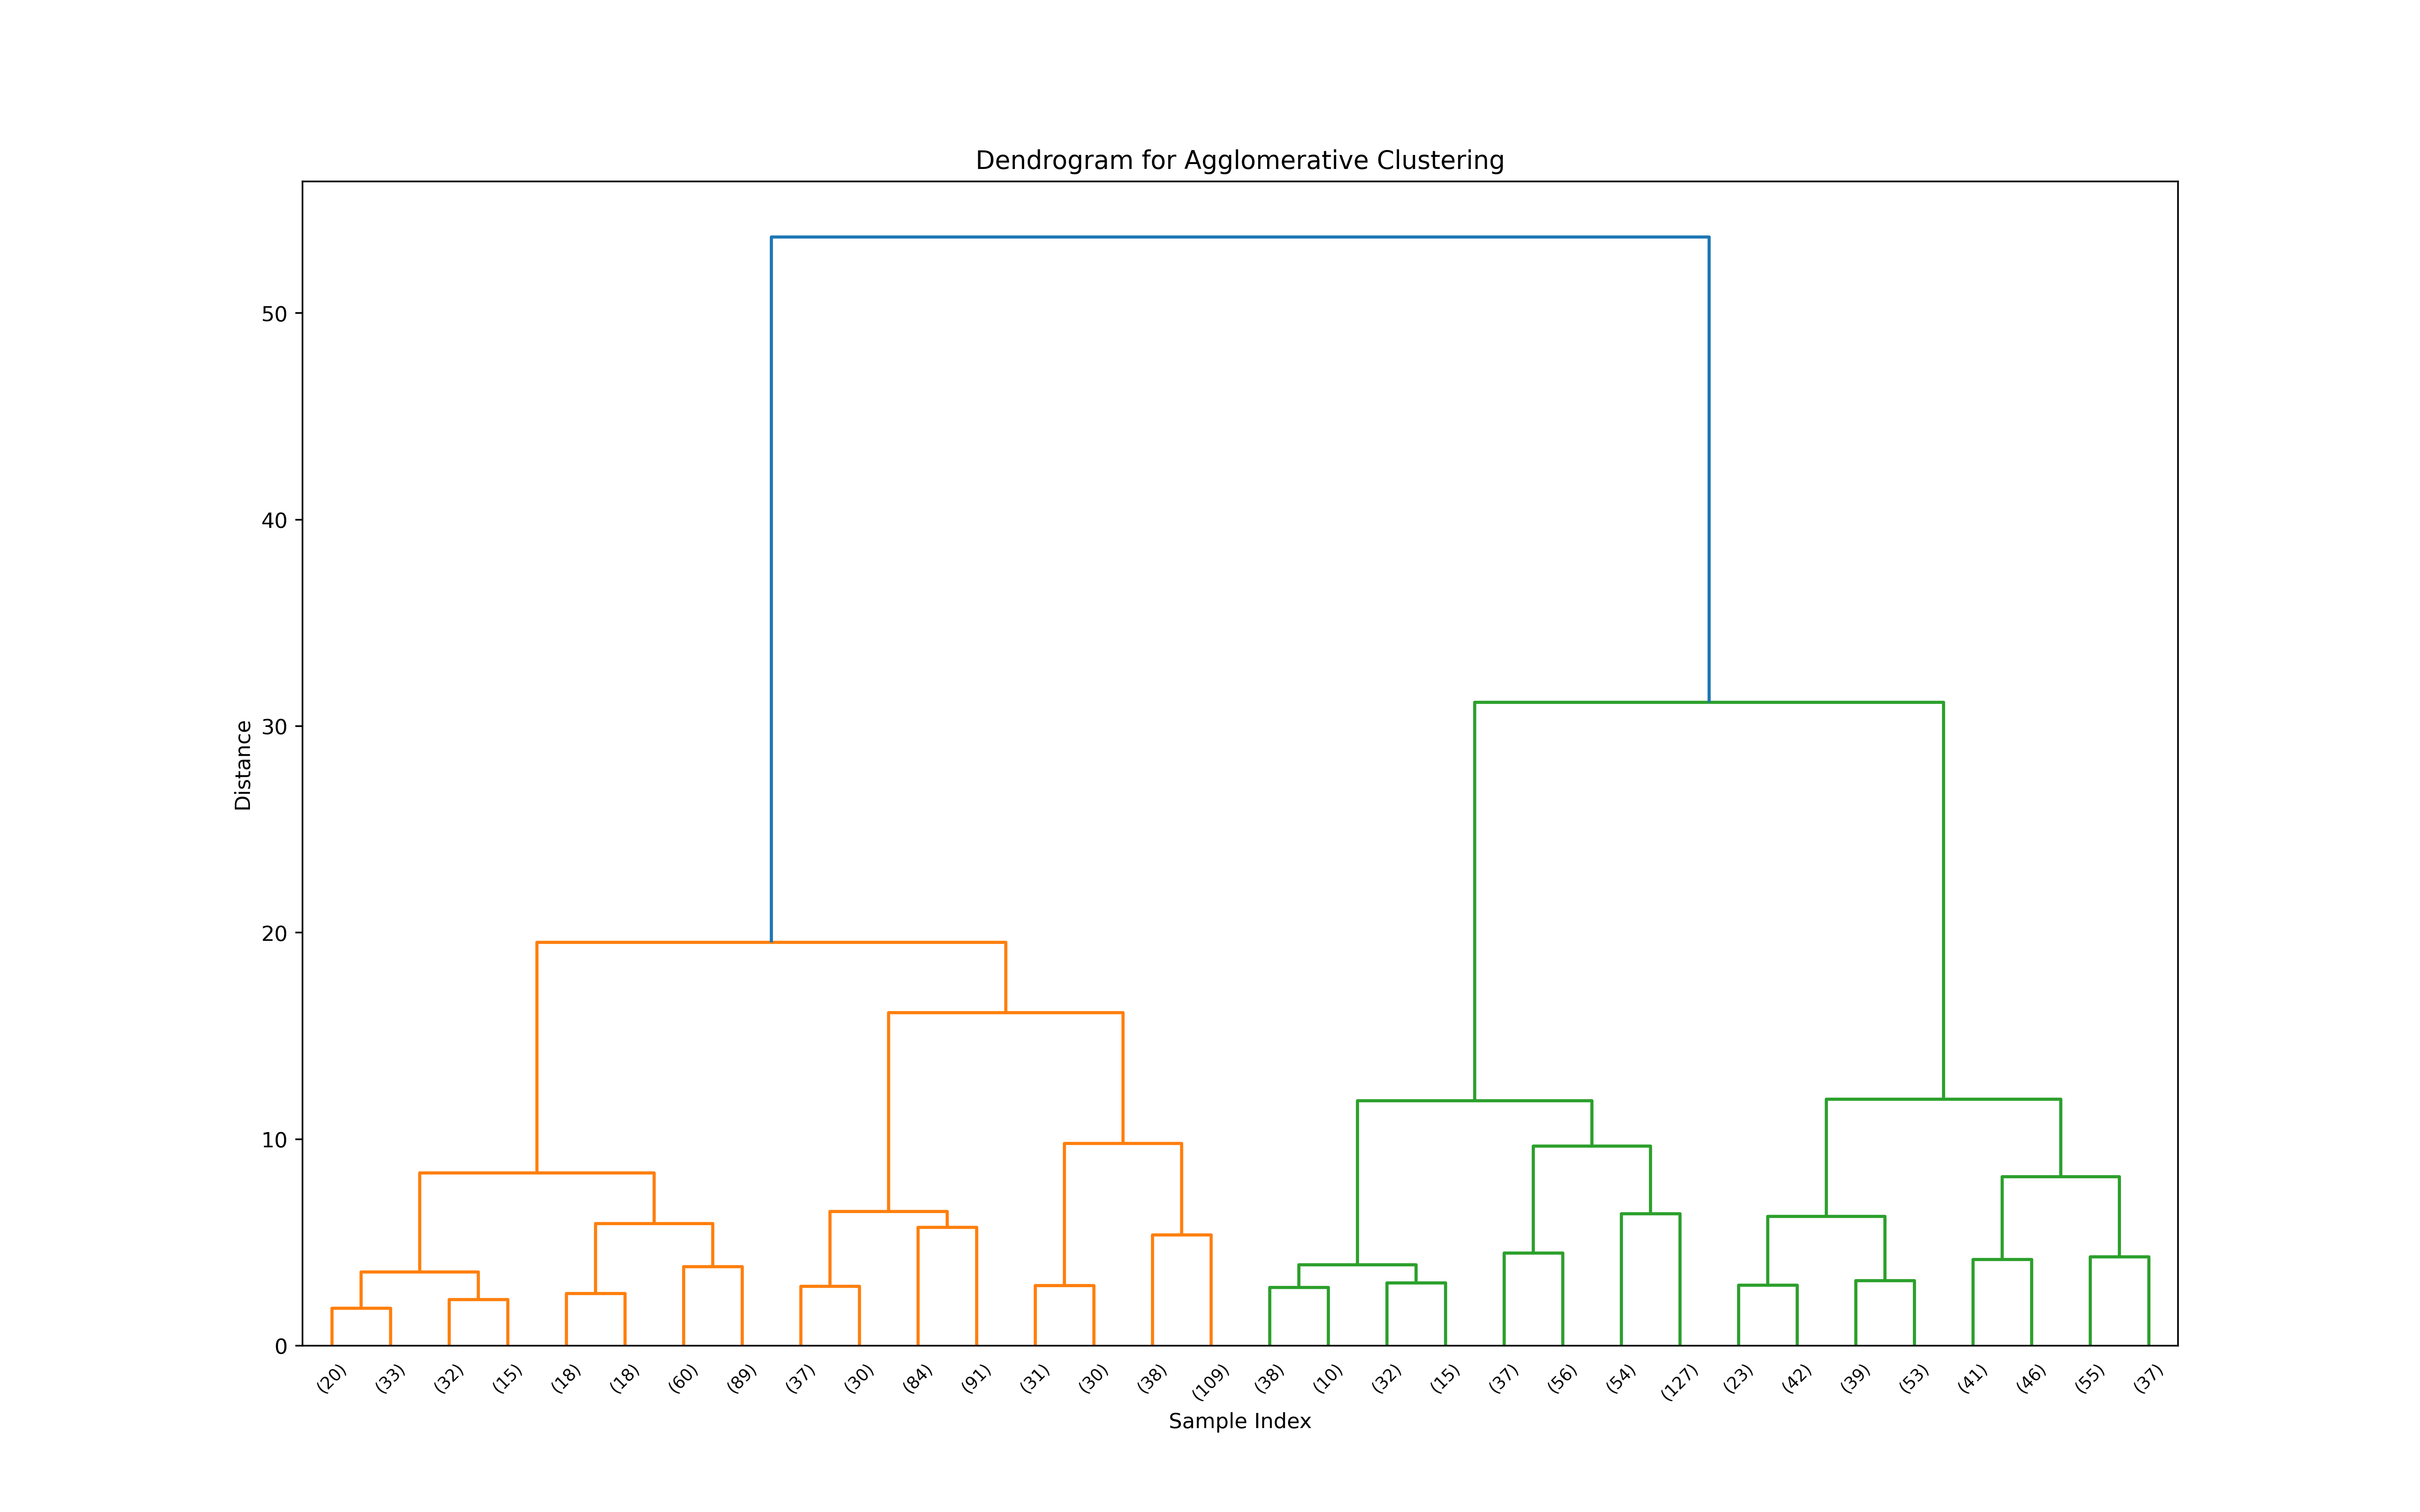
\includegraphics[width=0.75\linewidth]{Images/Clusters-5-v2-Agglomerative-Dendrogram.png}
    \caption{Dataset 3: Agglomerative Clustering Dendrogram}
    \label{fig:clusters-5-v2-agglomerative-dendrogram}
\end{figure}

\begin{figure}[H]
	\centering
	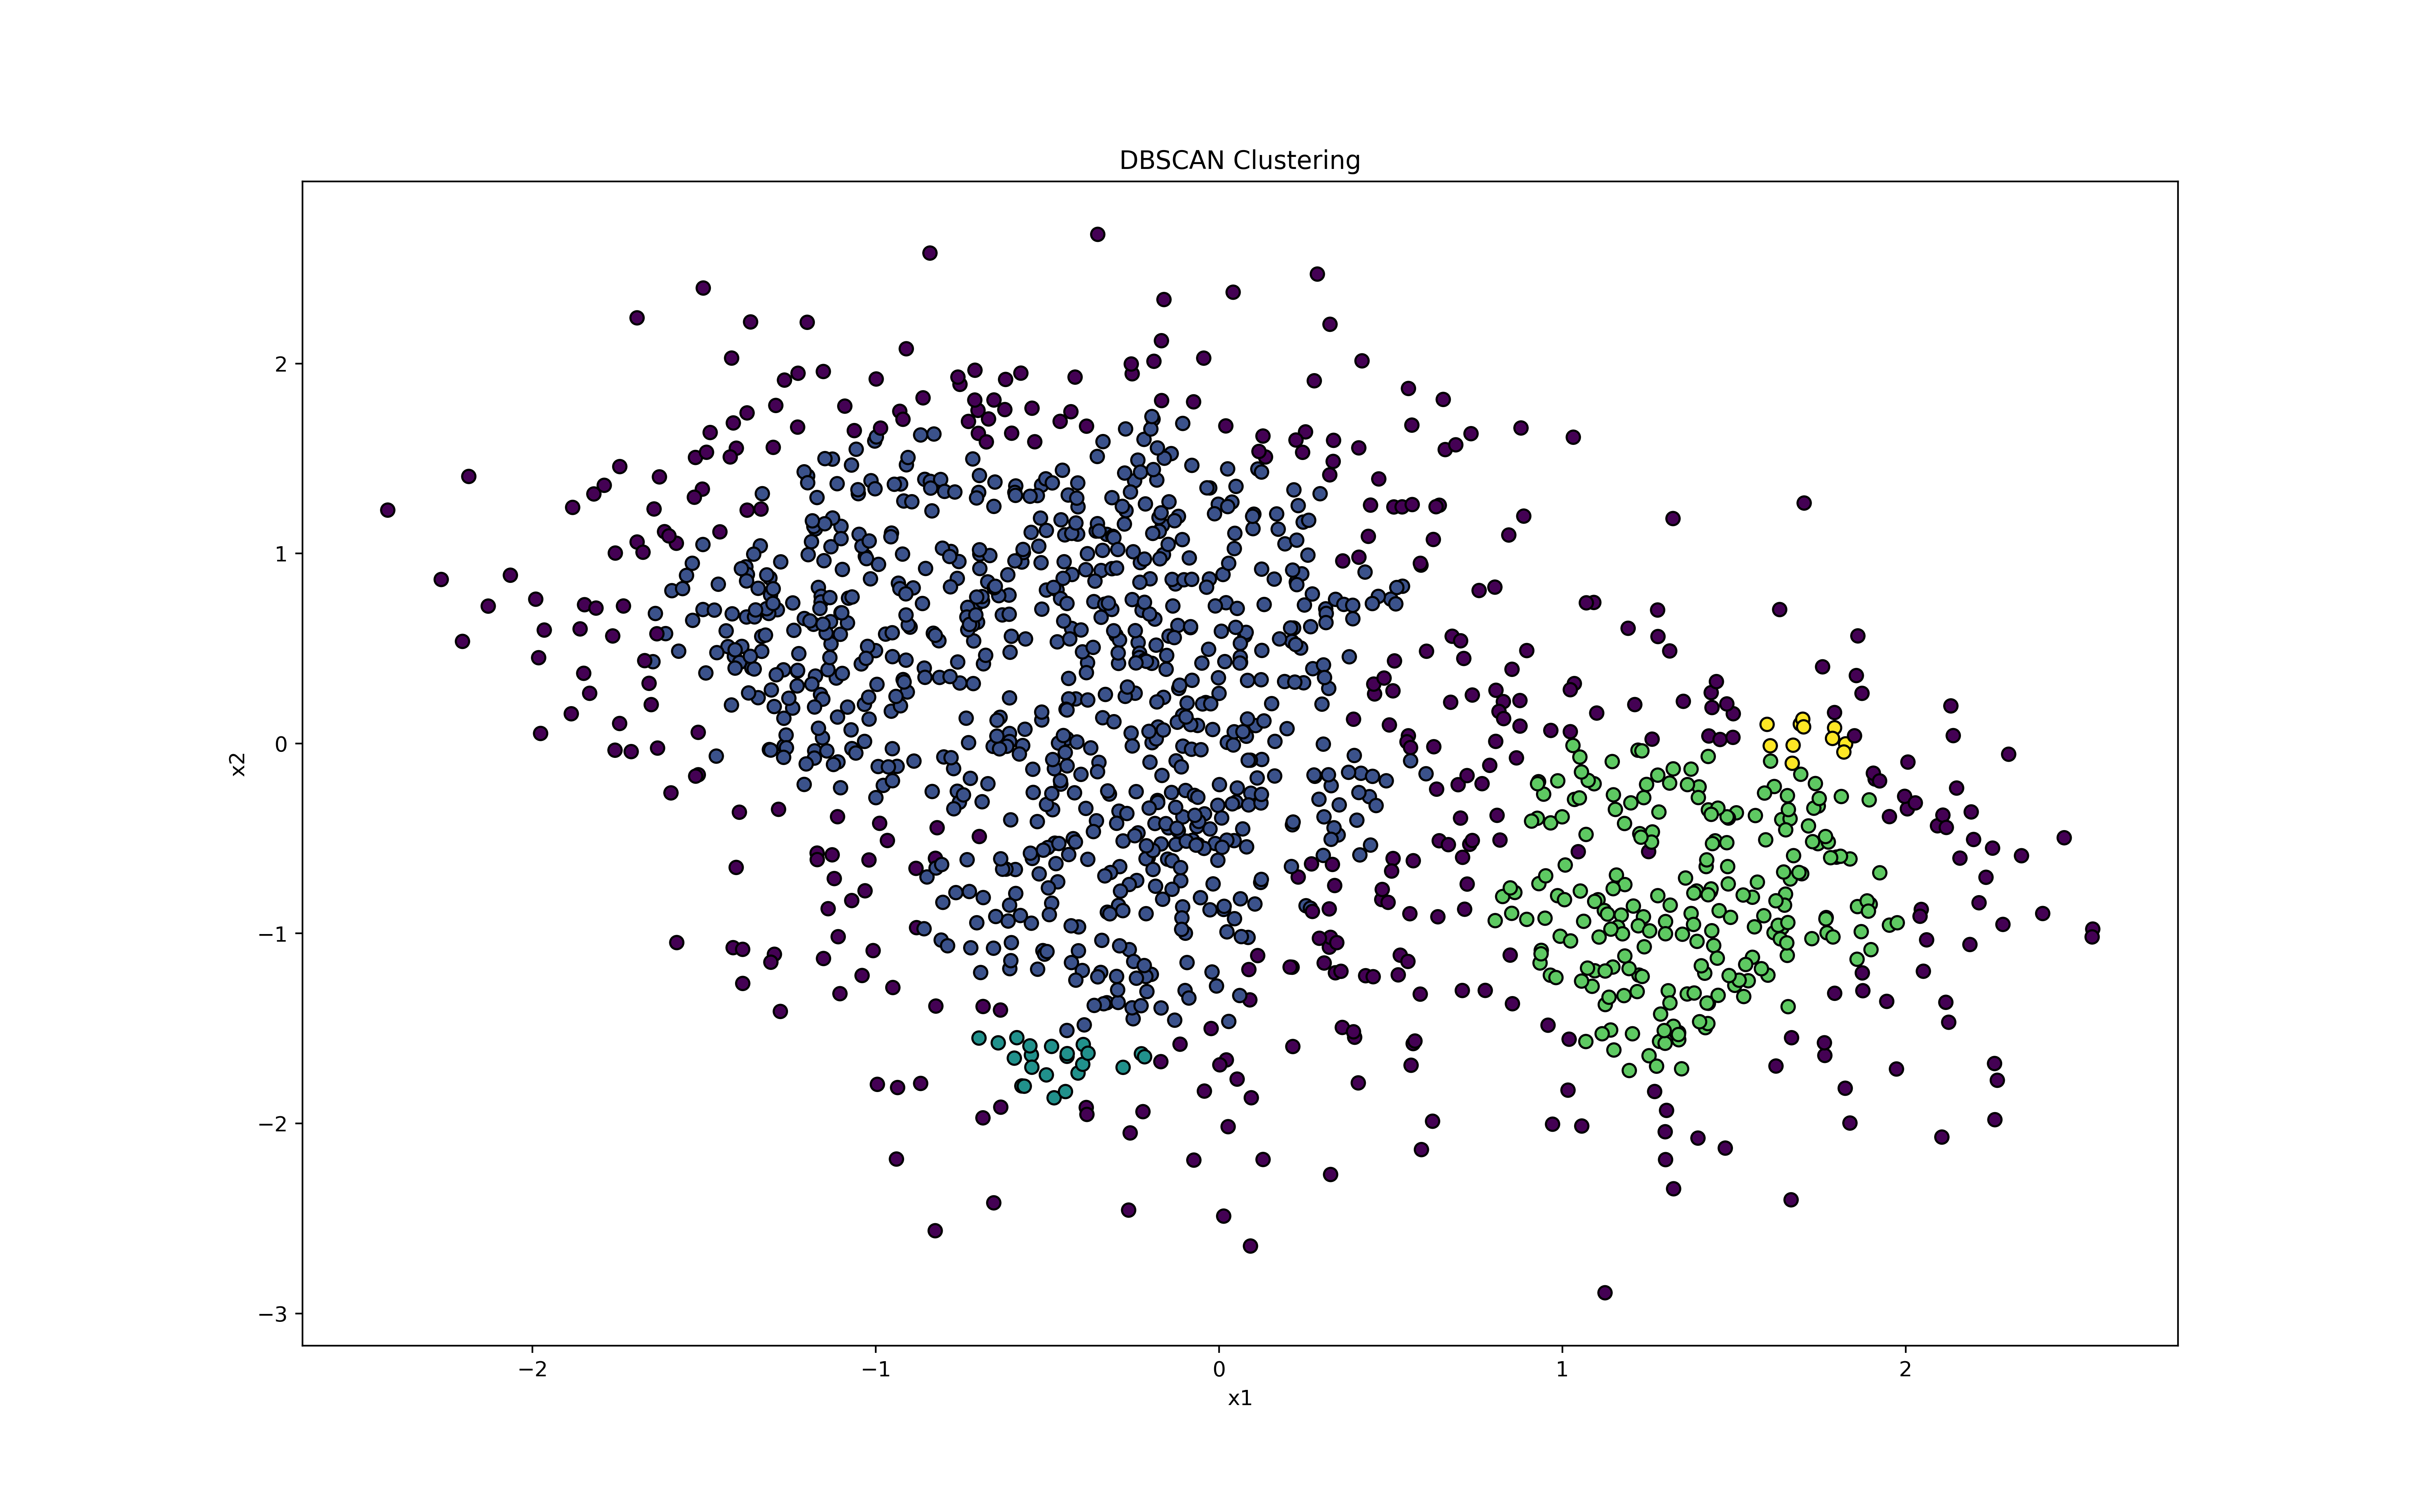
\includegraphics[width=0.75\linewidth]{Images/Clusters-5-v2-DBSCAN Clustering.png}
	\caption{Dataset 3: DBSCAN Clustering}
	\label{fig:clusters-5-v2-dbscan-clustering}
\end{figure}

For Dataset 3, we observe that none of the clustering algorithms have been able to cluster the observations effectively. The points are heavily overlapped and do not form distinct clusters. The DBSCAN algorithm has not been able to find exactly 4 clusters for this dataset. \\

The Silhouette Score for all three algorithms is close to 0, indicating that the points are on or very close to the decision boundary between clusters. This suggests that the clustering algorithms have not performed well for this dataset.

\clearpage